
\newcommand{\econtexRoot}{..}
\providecommand{\econtex}{./texmf-local/tex/latex/econtex}
\providecommand{\econtexSetup}{./texmf-local/tex/latex/econtexSetup}
\providecommand{\econtexShortcuts}{./texmf-local/tex/latex/econtexShortcuts}
\providecommand{\econtexBibMake}{./texmf-local/tex/latex/econtexBibMake}
\providecommand{\econtexBibStyle}{./texmf-local/bibtex/bst/econtex}
\providecommand{\notes}{./texmf-local/tex/latex/handout}
\providecommand{\handoutSetup}{./texmf-local/tex/latex/handoutSetup}
\providecommand{\handoutShortcuts}{./texmf-local/tex/latex/handoutShortcuts}
\providecommand{\handoutBibMake}{./texmf-local/tex/latex/handoutBibMake}
\providecommand{\handoutBibStyle}{./texmf-local/bibtex/bst/handout}

  
\documentclass[titlepage,abstract]{\econtex}\newcommand{\texname}{ctDiscrete}

\newcommand{\TabsDir}{\econtexRoot/Tables}\newcommand{\Calibration}{\econtexRoot/Calibration}


\usepackage{\econtexSetup}\usepackage{\econtexShortcuts}
\newcommand{\PTremark}[2][]{PT: {\it #2}}
\newcommand{\CDCremark}[2][]{CDC: {\it #2}}

\newenvironment{PTinserted}%
  {\noindent\ignorespaces\color{red}}%
  {\noindent\ignorespacesafterend}%

\newenvironment{CDCinserted}%
  {\noindent\ignorespaces\color{green}}%
  {\noindent\ignorespacesafterend}%

\newenvironment{PTmodified}%
  {\noindent\ignorespaces\color{red}}%
  {\noindent\ignorespacesafterend}%

\newenvironment{CDCmodified}%
  {\noindent\ignorespaces\color{red}}%
  {\noindent\ignorespacesafterend}%

\newcommand\PTcrossedout[1]{\color{red}{\sout{#1}}\color{black}}
\newcommand\CDCcrossedout[1]{\color{red}{\sout{#1}}\color{black}}

\let\PTdeleted\comment
\let\CDCdeleted\comment

% immature stuff
\newcommand{\done}{\ding{52}}
\newcommand{\notdone}{\ding{56}}
\newcommand{\cut}{\ding{36}}
\newcommand{\love}{\ding{170}}


% Nice tables
%\usepackage{booktabs}%defines\tabcolsep

% Modify commands defined in CDCShortcuts.sty
\renewcommand{\tSS}{}
    %\providecommand{\tSS}{\ensuremath{t}}
\renewcommand{\urate}{\ensuremath{\mu}}
    %\providecommand{\urate}{\ensuremath{\mho}}
\renewcommand{\erate}{(1-\urate)}
    %\providecommand{\erate}{\ensuremath{\cancel{\mho}}}
\renewcommand{\mLev}{\ensuremath{m}}
    %\providecommand{\mLev}{\ensuremath{\pmb{m}}}
    \renewcommand{\cLev}{\ensuremath{c}}
        %\providecommand{\cLev}{\ensuremath{\pmb{c}}}
\renewcommand{\aLev}{\ensuremath{a}}
    %\providecommand{\aLev}{\ensuremath{\pmb{a}}}
\renewcommand{\bLev}{\ensuremath{b}}
    %\providecommand{\bLev}{\ensuremath{\pmb{b}}}
\renewcommand{\mTarg}{\ensuremath{m}}
\newcommand{\nablaTarg}{\ensuremath{\nabla}}
\renewcommand{\aleph}{\ensuremath{\psi}}
\newcommand{\CEA}{\textsc{cea}}
\newcommand{\EU}{\textsc{eu}}
\newcommand{\VectorX}{\ensuremath{\pmb{X}}}
\newcommand{\VectorCoeff}{\ensuremath{\pmb{\gamma}}}

\usepackage{txfonts}


\pdfinclusioncopyfonts=1% graphics fonts included even if available on disk
                        % fonts on disk with same name might be different


\hypersetup{
            pdfauthor={Christopher D. Carroll <ccarroll@jhu.edu> and Patrick Toche <contact@patricktoche.com>},
            pdftitle={A Tractable Model of Buffer Stock Saving},
            pdfkeywords={risk, uncertainty, precautionary saving, buffer stock saving},
            pdfcreator = {ccarroll@jhu.edu}
            }

\newboolean{PDF}%
\setboolean{PDF}{true}%
\ifdvi\setboolean{PDF}{false}\fi%
\ifthenelse{\boolean{PDF}}{%
    \renewcommand{\baselinestretch}{1.2}%line spacing
}{}%


\begin{document}\bibliographystyle{\econtexBibStyle}

\hfill{\tiny \texname}%
\hfill{\tiny CDC response to PT edits for EJ resubmission}%

\title{A Tractable Model of Buffer Stock Saving}%

\begin{verbatimwrite}{\texname.title}
A Tractable Model of Buffer Stock Saving
\end{verbatimwrite}

\author{Christopher D. Carroll\authNum \and Patrick Toche\authNum}%

\keywords{risk, uncertainty, precautionary saving, buffer stock saving}%

\jelclass{C61, D11, E24}%

\maketitle%


\begin{abstract}%
  We present an analytically tractable model of the effects of
  nonfinancial risk on intertemporal choice. Our framework can be
  adopted in contexts where modelers have until now chosen not to
  incorporate serious nonfinancial risk because the available methods
  did not yield transparent insights.  Our model produces an
  intuitive formula for target assets, and we show how to analyze
  transition dynamics using a familiar Ramsey-style phase diagram.
  Despite its starkness, the model captures many of the key
  implications of nonfinancial risk for intertemporal choice.
\end{abstract}%


\vspace{0.15in}

\begin{small}
\parbox{\textwidth}{
\begin{center}
\begin{tabbing} 
\texttt{Archive:~} \= \= \url{http://econ.jhu.edu/people/ccarroll/papers/ctDiscrete.zip} \kill \\  
\texttt{~~~~PDF:~} \> \> \url{http://econ.jhu.edu/people/ccarroll/papers/ctDiscrete.pdf} \\
\texttt{~~~~Web:~} \> \> \url{http://econ.jhu.edu/people/ccarroll/papers/ctDiscrete/}    \\ 
\texttt{Archive:~} \> \> \url{http://econ.jhu.edu/people/ccarroll/papers/ctDiscrete.zip} \\
\texttt{~~~~~~~~~} \> \> {\it (Contains Mathematica and Matlab code solving the model)}
\end{tabbing}
\end{center}
}
\end{small}

\begin{authorsinfo}
\name{Carroll: \href{mailto:ccarroll@jhu.edu}{\texttt{ccarroll@jhu.edu}}, Department of Economics, Johns Hopkins University, Baltimore Maryland 21218, USA; and National Bureau of Economic Research.  \url{http://econ.jhu.edu/people/ccarroll}
\name{Toche: \href{mailto:contact@patricktoche.com}{\texttt{contact@patricktoche.com}}, Christ Church, Oxford OX1 1DP, UK.}}
\end{authorsinfo}%

\thanks{Thanks to several generations of Johns Hopkins University graduate students who helped correct many errors and infelicities in earlier versions of the material presented here.}%

\titlepagefinish%

\section{Introduction} 
The Merton-Samuelson model of portfolio choice is the foundation fo
the vast literature analyzing financial
risk,\footnote{\cite{merton:restat}; \cite{samuelson:portfolio}; see
  \cite{Sethi:Thompson:2000} for an overview and extensions.}  not
because it offers conclusions that cannot be obtained from othe
frameworks,\footnote{Merton and Samuelson cite the pioneering work of
  \cite{markowitz}, \cite{tobinRisk}, and \cite{phelpsRisk} among
  others whose work had already contained many of the important
  qualitative insights.} but because it is easy to use and its key
insights emerge in a way that is natural, transparent, and intuitive
--- in a word, the Merton-Samuelson model is tractable.

Unfortunately, nonfinancial risk\footnote{By which we mean risk that
  is both imperfectly insurable and imperfectly correlated with
  financial risk.} (which is much more important than financial risk
for most households)\footnote{Nonfinancial income typically accounts
  for the great majority of most households' total income, while risky
  assets like stocks represent a relatively small percentage of total
  wealth. Furthermore, stock returns are poorly correlated with the
  return on the index portfolio of all the assets in the economy.
  Idiosyncratic risk is even more poorly spanned by market risk and is
  several orders of magnitude greater than aggregate risk
  (\cite{Jagannathan:Kubota:Takehara:1998}).}  has proven more
difficult to analyze.  Of course, a large and impressive numerical
literature has carefully computed the effects of specific nonfinancial
risks in a variety of particular contexts.\footnote{The literature on
  in heterogeneous-agents macroeconomic models includes, among many
  others, \cite{carroll:brookings}, \cite{aiyagari:ge}, and
  \cite{ksHetero}, with roots that go back to
  \cite{schectman&escudero:results} and \cite{bewleyPIH}, with othe
  important contributions by \cite{clarida:ergodic},
  \cite{zeldesStochastic}, and \cite{cw:cUnderUncert}.}  But because the
computational methods necessary to solve such models are daunting and
the insights that emerge are not easy to explain, much of the economic
literature (and much graduate-level instruction) has dodged the
question of how nonfinancial risk influences choices, by assuming
perfect insurance markets or perfect foresight or risk neutrality o
quadratic utility or Constant Absolute Risk Aversion, or by attempting
only to match aggregate risks (which are orders of magnitude smalle
than idiosyncratic risks).  These approaches rob the question of its
essence, either by assuming (counterfactually) that markets transform
nonfinancial risk into financial risk or by making implausible
assumptions crafted to generate the implausible conclusion
that decisions are largely or entirely unaffected by nonfinancial
risk.\footnote{The case of CARA utility with only labor income risk is
  included here because \cite{carroll&kimball:concavity} show that it
  is a knife-edge case that is unrepresentative of the broader effects
  of uncertainty (notably, it fails to exhibit the consumption
  concavity that holds for virtually every other combination of
  assumptions); indeed, the addition of rate-of-return risk renders
  the optimal consumption function concave even under CARA utility.
  (The other traditional objection is that the optimal consumption
  plan under CARA utility generally involves setting consumption to a
  negative value in some states of the world; it is hard to think of a
  plausible economic interpretation of negative consumption.)}

Our contribution is to offer a tractable model that captures the main
features of realistic models of the optimal response to nonfinancial
risk, but without the customary technical difficulties. The model is a
natural extension of the no-risk perfect foresight framework. Its
solution is characterized by simple, intuitive equations and we show
how the model's results can be analyzed using a phase diagram like
that of the canonical Ramsey growth model.

The trick that yields tractability is to distill all nonreturn risk
into a stark and simple possibility: A one-time uninsurable permanent
loss in nonfinancial income.  Our view is that the consumer's response
to this single, tractable risk captures most of the substantive
essence of the results obtained by the numerical literature under more
realistic but more complex assumptions about income dynamics.  Indeed, our view is that ou
model matches essentially all of the qualitative and even some of the
quantitative implications of such models.
 
The kind of real-world shock that our $\urate$ shock most closely
resembles is permanent disability from which no recovery is possible.
We take the liberty of interpreting the shock more loosely, as
capturing the role of unemployment or forced retirement risk, fo
several reasons.  Most importantly, compared to perfect foresight
models, the key qualitative characteristic that distinguishes models
with a meaningful precautionary motive is the concavity of the
consumption function (see \cite{carroll&kimball:concavity} for general
proof that uncertainty induces consumption concavity), which ou
model generates in the simplest way we know of.  While exact
quantitative details of the consumption function generated by models
with more realistic formulations of income dynamics will differ from
those we obtain, our purpose here is more qualitative and analytical
than quantitative and empirical.\footnote{The reader might also be reassured
to know that the model could be modified without too much difficulty
to accommodate a multi-phase life cycle in which the risk applies only
in the last phase of life, in which it can be interpreted as the
probability of forced early retirement.  But such an extension would
add complexity and opacity to our exposition and notation, undermining
the paper's chief virtue, which is the transparency of its results.}

The same framework could be interpreted to apply in other contexts as well; for instance,
the risk faced by a country whose exports are dominated by a commodity
whose price might collapse permanently (e.g., oil exporters, if cold
fusion had worked).\footnote{ The model could even be interpreted as
  applying to the behavior of a firm controlled by a risk-neutral
  manager, so long as the collapse of a line of business could have
  the effect of reducing the firm's collateral value and therefore
  increasing its cost of external finance \textit{\`{a} la}
  \cite{bernanke&gertler&gilchrist:accellerator}. In this case, the
  convex increase in borrowing rates when cash drops plays the same
  role as the convexity of the marginal utility function for a
  consumer; see also \cite{bszHumK} for an argument that senior firm
  managers are not risk neutral even if shareholders are, because poo
  performance under their tenure will reduce their own future
  employment opportunities.  A firm controlled by such managers may
  behave very much like a risk-averse household.}

The optimal response to any such risk is to aim to accumulate a buffe
stock of precautionary assets.  The existing literature has computed the
numerical value of the target under specific parametric assumptions,
but has struggled to present an intuitive picture of the determinants
of that target.  Here, we are able to derive an analytical
formula for the target level of wealth, and show how the
precautionary motive (nonlinearly) interacts with the other saving motives that have
been well understood since Irving \cite{fisherInterestTheory}'s work:
The income, substitution, and human wealth effects.

\begin{comment}
This numerical literature has now almost entirely replaced an olde
approach (dating back to \cite{Skinner1988}) that attempted to address
the role of precautionary motives by approximating the nonlinear part
of the logarithmic consumption Euler equation (the part that drives
precautionary saving and the target level of assets).  
\end{comment}

Thanks to the model's tractability, we are able to derive a simple
expression that shows how the familiar perfect-foresight consumption
Euler equation is modified by the presence of our risk.  The effect of our risk on consumption growth
is related to the probability of the risky event, to its magnitude, to
the consumer's degree of risk aversion, to the consumer's wealth, and
to all of the parameters of the model (including risk aversion and
time preference). We obtain an exact analytical expression (not a
log-linearized one) for the combined value of the higher-order Euler equation terms
at the target.

With this expression in hand, the intuition for why empirical Euler equation
estimation is problematic comes into clear focus, and the problems that have
bedeviled the Euler equation literature can be plainly articulated and
understood (see section \ref{sec:death}).


A tractable model like ours can be used as a reference point for more
specialized models, complementing the perfect foresight, certainty
equivalent, or perfect markets models that are currently so widely
used because of their tractability. Even computation-intensive
literatures like heterogeneous-agents macroeconomics may find ours a
useful `toy model' with which to exposit some of the
subtle points that numerical simulations deliver without
interpretation.\footnote{In order to assist authors in modifying ou
  model for other purposes, we have constructed a public archive that
  contains Matlab and Mathematica programs that produce all the
  results and figures reported in this paper, along with some othe
  examples of uses to which the model could be put.  The archive is
  available on the first author's website.}

  If the consequences of nonfinancial risk were numerically
  trivial, a tractable model would be of little interest.  But the
  success of the growing heterogeneous-agents literature in
  macroeconomics suggests that the profession is increasingly coming
  to the view that something essential is missed when idiosyncratic
  risk is ruled out.

  Part, at least, of what is missing in such models is the ability to
  analyze the consequences of wealth heterogeneity.  In the absence of
  nonfinancial risk, \cite{uzawa:patientownall} pointed out that if
  infinite-horizon agents have heterogeneous preferences, the most
  patient agent ends up owning all aggregate wealth in equilibrium (a point 
that was anticipated, but not fully developed, in \cite{ramsey:save} and is
fleshed out in \cite{beckerWealth}).  
  Mathematically, this is because any agent who is impatient (at the
  prevailing interest rate) will choose to run down his wealth to its
  minimum possible value, while any agent who is patient relative to
  that interest rate will choose to accumulate indefinitely.
  

  If we grant that there is even a small amount of heterogeneity in
  time preference rates, relative risk aversion, expected income
  growth, mortality risk, age, or any other factor that influences
  intertemporal choice, a model without nonfinancial risk leads to
  radical wealth inequality that is even greater than 
  the substantial but not unlimited differences in wealth in the
  cross-sectional data.
  

  In such a world, the representative agent model's approximation of
  behavior around the aggregate steady-state wealth-to-income ratio is
  an approximation around a wealth-to-income ratio that is arbitrarily
  far from the wealth-to-income ratio that anyone in the economy will
  actually experience.  To take a simple example, suppose everybody
  has the same nonfinancial income, borrowing is ruled out, and
  suppose that 5 percent of agents are ``patient'' and 95 percent are
  ``impatient.''  Then the patient agents will have a wealth-to-income
  ratio equal to about 20 times the aggregate ratio, while impatient
  agents will have a wealth-to-income ratio of zero.  Since no
  approximation is good at vast distances from the approximating
  point, there is no reason to suppose that approximating behavio
  around the aggregate wealth-to-income ratio will provide even a
  remotely accurate description of the behavior of the actual
  aggregate economy with heterogeneous agents but perfect foresight.
  Indeed, the logic of the model is that essentially {\it nobody} will
  hold a level of wealth close to the representative agent's level of
  wealth, around which {\it everybody's} behavior is approximated.

  The appeal of introducing nonfinancial risk is that the
  precautionary motive prevents wealth from asymptoting to its lowe
  bound for households who are impatient relative to the interest
  rate.  Each kind of household's behavior can be approximated around
  a target level of wealth that reflects their actual wealth, rathe
  than around the representative agent's wealth.  In the presence of 
heterogeneity and nonfinancial risk, the only agents whose behavior is
{\it not} captured by the model are those who are patient relative to the equilibrium interest rate.  Since the wealth of those agents is heading to infinity, 
their behavior may be reasonably approximated by the behavior of a perfect foresight
agent.


\section{The Decision Problem}
For concreteness, we analyze the problem of an individual consume
facing a labor income risk.  Other interpretations (like those
mentioned in the introduction) are left for future work or othe
authors.\footnote{See \cite{toche:urisk} for an explicit but brief treatment 
  of a closely related model in continuous time.}

The aggregate wage rate, $\Wage_{t},$ grows by a constant factor $\WGroPF$ from the current time period to the next, reflecting exogenous productivity growth:
\begin{eqnarray}
        \Wage_{t+1} & = & \WGroPF \Wage_{t}.
\end{eqnarray}

The interest rate is exogenous and constant (the economy is small and open); the interest factor is denoted $\Rfree$.\footnote{General equilibrium is not much more difficult; it requires specifying a production function and finding the level of capital for which the optimal level of saving is zero (net of depreciation).  Little further insight is obtained, while several potential sources of confusion would be added.}
Define $\mLev$ as market resources (financial wealth plus current income), $\aLev$ as end-of-period assets after all actions have been accomplished (specifically, after the consumption decision), and $\bLev$ as bank balances before receipt of labor income. Individuals are subject to a dynamic budget constraint (DBC) that can be decomposed into the following elements:
\begin{eqnarray}
    \aLev_{t} & = & \mLev_{t}-\cLev_{t}
\\  \bLev_{t+1} & = & \Rfree \aLev_{t}
\\  \mLev_{t+1} & = & \bLev_{t+1}+\Wage_{t+1}\labor_{t+1}\empState_{t+1}  \label{eq:DBC}
\end{eqnarray}
where $\labor$ measures the consumer's labor productivity (hours of
work for an employed consumer are assumed to be exogenous and fixed)
and $\empState$ is a dummy variable indicating the consumer's
employment state: Everyone in this economy is either employed
($\empState = 1$, a state indicated by the letter `e') or unemployed
($\empState=0$, a state indicated by `u'). Thus, labor income is zero
for unemployed consumers.\footnote{This is without loss of generality.  On
  this, see also footnote~4 in~\cite{toche:urisk}.}



\subsection{The Unemployed Consumer's Problem}
There is no way out of unemployment; if an individual becomes
unemployed, that individual remains unemployed forever,
$\empState_{t}=0 \implies \empState_{t+1}=0~\forall~t$.  
\subsubsection{The Consumption Function }
Consumers have a CRRA utility function
$\uFunc(c)=c^{1-\CRRA}/(1-\CRRA)$, with $\CRRA>1$, and 
they discount future utility geometrically by $\Discount$ pe
period.  We show below that the simplicity of the unemployed consumer's behavior is what makes employed consumer's problem tractable. 
The solution to the unemployed consumer's optimization problem
is simply:\footnote{This is a standard result, which follows from the first-order condition and the budget constraint:
\begin{eqnarray*}
\uFunc^{\prime}(\cLevU_{t}) = \Rfree\Discount \uFunc^{\prime}(\cLevU_{t+1})
\Rightarrow \
\left(\cLevU_{t}\right)^{-\CRRA} = \Rfree\Discount \left(\cLevU_{t+1}\right)^{-\CRRA} 
\Rightarrow \
\cLevU_{t+1} = \left(\Rfree\Discount\right)^{1/\CRRA} \cLevU_{t}
.
\end{eqnarray*}
Consumption grows at the geometric rate $\left(\Rfree\Discount\right)^{1/\CRRA}$. The present discounted value of consumption at time $t$ must equal total wealth, so that
\begin{eqnarray*} 
\sum_{i=0}^{\infty} R^{-i} \cLevU_{t+i} = \sum_{i=0}^{\infty} R^{-i} \left(\Rfree\Discount\right)^{i/\CRRA} \cLevU_{t} = \sum_{i=0}^{\infty} (1-\MPCU)^{i} \cLevU_{t} = \cLevU_{t} / \MPCU =  \bLev_{t}.
\end{eqnarray*}
}
\begin{eqnarray}
  \cLevU_{t} & = & \MPCU \bLev_{t} 
\label{eq:cpfinfhorunemp}
\label{eq:cdel}
\label{eq:kappaDef}
,
\end{eqnarray}
where 
\begin{eqnarray}
  \MPCU = 1 - \Rfree^{-1}(\Rfree{\Discount})^{1/\CRRA}
\label{eq:MPCU}
.
\end{eqnarray}
$\MPCU$ is the `marginal propensity to consume' out of total wealth
(MPC), which for the unemployed consists in bank balances $\bLev$ only, 
because we have assumed that noncapital income of the unemployed is
zero.  This is for simplicity only; incorporation of an unemployment
insurance system that pays a fixed proportion of the final employed
wage is straightforward, because in the absence of furthe
uncertainty the value of those future payments is equivalent to
receipt of a lump sum equal to the present discounted value of the
payments.  The accompanying solution code for the model, in fact,
incorporates a parameter measuring the generosity of the
unemployment insurance system, and the solutions presented in the
paper are those produced when that parameter is set to zero.


\subsubsection{Parameter Restrictions\label{sec:params1}}
Table~\ref{table:notation} summarizes our notation. We follow the terminology in \cite{BufferStockTheory}, where a detailed discussion of the concepts is provided. 
We impose a condition on parameters to ensure that the marginal propensity to consume out of total wealth is positive, $\MPCU>0$:
\begin{eqnarray}
(\Rfree \Discount)^{1/\CRRA} & < & \Rfree.
\label{eq:RIC}
\end{eqnarray}
The unemployed consumer will be spending enough to make the ratio of financial wealth to human wealth decline over time. The interpretation is that the consumer must not be so patient that a boost to wealth would fail to boost current consumption. An alternative (equally correct) interpretation is that the condition guarantees that the present discounted value (PDV) of consumption for the unemployed consumer remains finite.\footnote{`Pathologically patient' consumers who do not satisfy this condition would hoard any increase in wealth in order to enable even more extra consumption in the distant future.}  

Note that our results do not depend on the stronger\footnote{Assuming $\Rfree \geq 1$.} restriction that is often imposed:
\begin{eqnarray}
\Rfree \Discount & < & 1.
\label{eq:ImPat}
\end{eqnarray}
Here the consumer will choose to spend more than the amount that would permit constant consumption; such a consumer's absolute level of wealth declines over time, together with consumption, since consumption and wealth are proportional. \cite{BufferStockTheory} calls the first type of consumer ``return impatient'' and the second, more impatient type ``absolutely impatient.'' The restriction we impose, therefore, is the Return Impatience Condition~(RIC) defined in \cite{carrollBSTheory}.



\subsection{The Employed Consumer's Problem}
The consumer's preferences are the same in the employment and unemployment states; only exposure to risk differs.
There are two effects at work. On the one hand, the precautionary saving motive is inversely related to wealth, so that `poor' consumers choose to save more than `rich' consumers. On the other hand, the impatience motive is independent of wealth. The two effects thus influence wealth in opposite directions. Under our parameter restrictions, there is a point at which prudence and impatience are in exact balance. This balance condition defines the target wealth-to-income ratio.

\subsubsection{A Human-Wealth-Preserving Spread in Unemployment Risk}
A consumer who is \textit{employed} in the current period has $\empState_{t}=1$; if this person is still employed next period ($\empState_{t+1}=1$), market resources will be:
\begin{equation}
\mLevE_{t+1} = \Rfree(\mLevE_{t}-\cLevE_{t})+\Wage_{t+1}\labor_{t+1} \label{eq:Metp1}
.
\end{equation}
However, there is no guarantee that the consumer will remain employed: Employed consumers face a constant risk $\urate$ of becoming unemployed.  

We assume that $\labor$ grows by a factor $(1-\urate)^{-1}$ every period,
\begin{equation}
\labor_{t+1} =    \labor_{t}/(1-\urate) 
\label{eq:meanPreserve}
,
\end{equation}
because under this assumption, for a consumer who remains employed, labor income will grow by factor $\PGro=\WGroPF/(1-\urate)$,
so that the \textit{expected} labor income growth factor for employed consumers is the same $\WGroPF$ as in the no-risk perfect foresight case:
\begin{eqnarray*}
   \Ex_{t}[\Wage_{t+1}\labor_{t+1}\empState_{t+1}] 
   & = &  
   \PGro \Wage_{t} \labor_{t} \left(\urate \times 0 + (1-\urate) \times 1 \right)
\\ 
\Rightarrow 
\frac{\Ex_{t}[\Wage_{t+1}\labor_{t+1}\empState_{t+1}]}{\Wage_{t} \labor_{t}} &  = & \PGro (1-\urate) = \WGroPF \hspace{20pt} = \text{no-risk growth}
\end{eqnarray*}
implying that an increase in $\urate$ is a pure increase in risk with
no effect on the PDV of expected labor income -- a mean-preserving
spread.  Thus, any change in behavior that
results from a change in $\urate$ is cleanly interpretable as
reflecting an effect of uncertainty rather than the effect of a change
in human wealth. For analytical convenience, we henceforth treat the risk-adjusted growth factor $\PGro$ as a parameter, rather than the `structural' parameter $\WGroPF$.


\subsubsection{First Order Optimality Condition}
The usual steps lead to the standard consumption Euler equation. Using $i \in \{e,u\}$ to stand for the two possible states,
\begin{eqnarray}
     \uFunc^{\prime}(\cLevE_{t}) & = & \Rfree\Discount \Ex_{t}\left[\uFunc^{\prime}(\cLev^{i}_{t+1}) \right] \nonumbe
\\
\Rightarrow \ 
   1         & = & \Rfree\Discount \Ex_{t}\left[\left(\frac{\cLev^{i}_{t+1}}{\cLevE_{t}}\right)^{-\CRRA} \right]
.
\end{eqnarray}

Henceforth nonbold variables will be used to represent the bold equivalent divided by the level of permanent labor income for an employed consumer, e.g.\ $\cRatE_{t}=\cLevE_{t}/(\Wage_{t}\labor_{t})$; thus we can rewrite the consumption Euler equation as:%\footnote{If your reader/printer does not render sharp bold letters, simply consider that henceforth all variables that grow in a steady state have been scaled by labor income $\Wage_{t}\labor_{t}$. }
\begin{eqnarray}
  1         & = & \Rfree\Discount \Ex_{t}\left[\left(\frac{\Wage_{t+1}\labor_{t+1}{c}^{i}_{t+1}}{\Wage_{t}\labor_{t}\cRatE_{t}}\right)^{-\CRRA} \right]
\nonumber%\label{eq:ceuler}
\\
\Rightarrow \
  1        & = & \Rfree\Discount \Ex_{t}\left[\left(\PGro \ \frac{{c}^{i}_{t+1}}{\cRatE_{t}}\right)^{-\CRRA} \right] \nonumbe
\\
\Rightarrow \
  1        & = & \Rfree\Discount\PGro^{-\CRRA} \left\{(1-\urate)\left(\frac{\cRatE_{t+1}}{\cRatE_{t}}\right)^{-\CRRA}+\urate \left(\frac{\cU_{t+1}}{\cRatE_{t}}\right)^{-\CRRA}\right\}
\label{eq:Explicit}
,
\end{eqnarray}
where the term in braces is a probability-weighted average of the growth rates of marginal utility in the case where the consumer remains employed (the first term) and the case where the consumer becomes unemployed (the second term).


\subsubsection{Analysis and Intuition of Consumption Growth Path}


An intuitive interpretation of the consumption Euler equation is readily available. Re-write equation~\eqref{eq:Explicit} in terms of the growth rate of consumption in the employment state:
\begin{eqnarray}
  \left(\frac{\cRatE_{t+1} \PGro}{\cRatE_{t}}\right)  = \left(\frac{\cLevE_{t+1}}{\cLevE_{t}}\right) 
  & = & 
  \Pat \left\{1+\urate\left[\left(\frac{\cRatE_{t+1}}{\cU_{t+1}}\right)^{\CRRA}-1\right]\right\}^{1/\CRRA}
\label{eq:cedel}
,
\end{eqnarray}
where 
\begin{eqnarray}
\Pat = (\Rfree\Discount)^{1/\CRRA}
\label{eq:PatPGro}
\end{eqnarray}
is the factor by which the level of consumption $\cLev$ would grow in a perfect foresight no-risk model. 

To understand~\eqref{eq:cedel}, it is useful to consider an
approximation.  Define $\nabla_{t+1} \equiv
\left(\frac{\cRatE_{t+1}-\cU_{t+1}}{\cU_{t+1}}\right)$, the proportion
by which the consumption ratio next period would be lower in the event of a
transition into unemployment; we refer to this loosely as the size of
the `consumption risk.' Define $\prudEx$, the `excess prudence'
factor, as $\prudEx = (\CRRA-1)/2$.\footnote{It is `excess' in the sense of exceeding the benchmark case of logarithmic utility which corresponds to $\CRRA=1$.  Logarithmic utility is often viewed as a lower bound on the possible degree of risk aversion.}
Applying a Taylor approximation to~\eqref{eq:cedel} (see appendix \ref{sec:cGroTaylor}) yields:
\begin{eqnarray}
  \left(\frac{\cLevE_{t+1}}{\cLevE_{t}}\right) & \approx & \left(1+ \urate (1+\prudEx\nabla _{t+1})\nabla _{t+1}\right) {\Pat}
\label{eq:cedelapprox}
,
\end{eqnarray}
which simplifies further in the logarithmic utility case (since $\CRRA = 1$ and thus $\prudEx = 0$) to
\begin{eqnarray}
  \left(\frac{\cLevE_{t+1}}{\cLevE_{t}}\right) & \approx & \left(1+ \urate \nabla _{t+1}\right) {\Pat}
\label{eq:cedelapproxLog}
.
\end{eqnarray}

The approximations in~\eqref{eq:cedelapprox} or~\eqref{eq:cedelapproxLog} capture the essence of equation~\eqref{eq:cedel}. As a consequence of missing insurance markets, consumption growth depends on the employment outcome; the consumption ratio if employed next
period $\cRatE_{t+1}$ is greater than if unemployed 
$\cRatU_{t+1}$, so that $\nabla _{t+1}$ is positive.
In the limit case, if we let the transition probability $\urate$ go to zero, consumption risk $\nabla$ vanishes and thus $\cLevE_{t+1}/\cLevE_{t}$ approaches its perfect-foresight value ${\Pat}$. Equation~\eqref{eq:cedelapprox} thus shows that the presence of unemployment risk boosts consumption growth by an amount proportional to the probability of becoming unemployed $\urate$ multiplied by a factor that is increasing in the amount of consumption risk $\nabla$. Equation~\eqref{eq:cedelapproxLog}
shows that, in the logarithmic case, the precautionary boost to consumption growth is directly proportional to the size of the consumption risk.

The effect of risk on saving is transparent. For a given value of $\mRatE_{t}$, risk has no effect (by construction) on the PDV of future labor income and human wealth, but the larger is $\urate$, the faster consumption growth must be, as equation~\eqref{eq:cedelapprox} shows.  For consumption growth to be faster while keeping its PDV constant, the \textit{level} of \textit{current} $\cLevE$ must be lower.  Thus, the introduction of a risk of unemployment $\urate$ induces a (precautionary) increase in saving.

In the (persuasive) case where $\CRRA > 1$, equation~\eqref{eq:cedelapprox} implies that a consumer with a higher degree of prudence (larger $\CRRA$ and therefore larger $\prudEx$) will anticipate greater consumption growth.  This reflects the greater precautionary saving motive induced by a higher degree of prudence.

\subsubsection{The Steady State}
To compute the steady state of the model, we explicitly solve for the $\Delta \cRatE_{t+1}=0$ and $\Delta \mRatE_{t+1}=0$ loci. 

Consider a consumer who is employed in period $t$ and at his steady-state target value of $\bRatE_{t}$. Substituting $\cRatE_{t+1} = \cRatE_{t} = \cRatE_{\tSS}$ and  $\cU_{t+1} =  \cU_{\tSS}$ into~\eqref{eq:cedel} and rearranging yields the ratio of consumption in the two states at the buffer-stock target value:
\begin{eqnarray}
  (\Pat/\PGro)^{-\CRRA}
  & = & 
  1+\urate
  \left[\left(\frac{\cRatE_{t+1}}{\cU_{t+1}}\right)^{\CRRA}-1\right]
\nonumber  
\\
\Rightarrow \
\frac{\cRatE_{\tSS}}{\cU_{\tSS}} 
& = & 
\left[\frac{(\Pat/\PGro)^{-\CRRA}-(1-\urate)}{\urate}\right]^{1/\CRRA}
\label{eq:cDelEqZero}
.
\end{eqnarray}
Next, the dynamic budget constraint~\eqref{eq:DBC} may be used to express $\cU_{\tSS}$ in terms of $\cRatE_{\tSS}$. If a transition into unemployment occurs at date $t$, then $\mLev_{t+1}^{u} = \bLev_{t+1}^{u} = \bLev_{t+1}^{e}$, implying:
\begin{eqnarray}
  \mLev_{t+1}^{u}
  & = & 
  \Rfree (\mLev_{t}^{e}-\cLev_{t}^{e})
\nonumber  
\\
\Rightarrow \
\frac{\mLev_{t+1}^{u}}{\Wage_{t+1}\labor_{t+1}}
  & = & 
\Rfree \left[\frac{\mLev_{t}^{e}}{\Wage_{t}\labor_{t}} - \frac{\cLev_{t}^{e}}{\Wage_{t}\labor_{t}}\right] \frac{\Wage_{t}\labor_{t}}{\Wage_{t+1}\labor_{t+1}}
\nonumber  
\\
\Rightarrow \
\mU_{t+1} 
  & = & 
 \Rfree (\mRatE_{t}-\cRatE_{t})/\PGro 
\nonumber  
\\
\Rightarrow \
\cU_{t+1} 
  & = & 
 \MPCU \Rfree (\mRatE_{t}-\cRatE_{t})/\PGro 
\nonumber  
\\
\Rightarrow \
\cU_{\tSS}
  & = & 
(\mRatE_{\tSS}-\cRatE_{\tSS}) \MPCU \Rfree/\PGro 
\label{eq:DBCnormalized}
\end{eqnarray}
where the consumption function~\eqref{eq:cdel} $\cLev_{t+1}^{u} =  \MPCU \mLev_{t+1}^{u}$ was used. Then, equations~\eqref{eq:cDelEqZero} and~\eqref{eq:DBCnormalized} may be solved for $\cRatE_{\tSS}$ in terms of $\mRatE_{\tSS}$; straightforward algebra shows that the $\Delta \cRatE_{t+1}=0$ locus is characterized by proportionality between $\cRatE_{\tSS}$ and $\mRatE_{\tSS}$:
\begin{eqnarray}
  \cRatE_{\tSS} & = & \pi \mRatE_{\tSS} 
\label{eq:DceEq0}
\end{eqnarray}
where
\begin{eqnarray}
  \frac{\pi}{1-\pi} & \equiv & \MPCU \left(\Rfree/\PGro\right) \left[\frac{(\Pat/\PGro)^{-\CRRA}-(1-\urate)}{\urate}\right]^{1/\CRRA}. \label{eq:DcSlope}
\end{eqnarray}
To characterize the $\Delta \mRatE_{t+1}=0$ locus, we normalize the budget constraint~\eqref{eq:DBC} for the employment state, paralleling the normalization for the unemployment state detailed in~\eqref{eq:DBCnormalized},
\begin{eqnarray}
  \mRatE_{t+1}  
  & = & 
  (\mRatE_{t}-\cRatE_{t}) \Rfree/\PGro + 1
\nonumber 
\\
\Rightarrow \
  \cRatE_{\tSS}  
  & = & 
  \frac{ 1 + (\Rfree/\PGro-1) \mRatE_{\tSS} }{\Rfree/\PGro}
\label{eq:xDelEqZero}
.
\end{eqnarray}
The target values $\mRatE$ and $\cRatE$ solve the linear system formed by equations~\eqref{eq:DceEq0} and~\eqref{eq:xDelEqZero}. 
Equation~\eqref{eq:DceEq0} is a steady-state version of the Euler equation of the employed worker, \textit{conditional upon remaining employed}, where the marginal utility in the unemployment state is expressed in terms of wealth. Note that while the steady-state condition is associated with a (hypothetical) steady state in which unemployment is never actually realized, the aversion to the risk of unemployment exerts an effect on that steady state. Equation~\eqref{eq:xDelEqZero} is a steady-state version of the budget constaint of the employed worker. To each steady-state condition is associated a locus used to depict the phase diagram of the system in Figure~\ref{fig:PhaseDiag}. The buffer-stock target ratio is given by the intersection of the two loci. Since the conditions are linear, the intersection is unique (our parameter restrictions ensure existence).

The appendix details the complete solution. Before we turn to an analysis of the target level of $\mRatE$, we briefly discuss parameter restrictions needed to ensure its existence.


\subsubsection{Parameter Restrictions (Continued)\label{sec:params2}}
In section \ref{sec:params1}, we derived a set of parameter restrictions from the problem of the unemployed consumer that ensure $\MPCU>0$ (the RIC). In this section, we derive a further set of restrictions from the problem of the employed consumer. The solution in employment is characterized by $\mRatE_{t} > \cRatE_{t} > 0$ because, with CRRA preferences, zero consumption carries an infinite penalty, implying that a consumer facing the risk of perpetual unemployment will never borrow. Therefore, as may be seen from equation~\eqref{eq:cDelEqZero}, steady-state consumption is positive only if:
\begin{eqnarray}
  \Pat/\PGro & < & (1-\urate)^{-1/\CRRA} 
\label{eq:PGroMod}
.
\end{eqnarray}
In the limit, as $\urate$ approaches zero, the condition reduces to $\Pat/\PGro<1$, or equivalently:
\begin{eqnarray}
(\Rfree\Discount)^{1/\CRRA}  & < & \PGro
\label{eq:GIC}
\end{eqnarray}
It is useful to compare condition~\eqref{eq:GIC} with condition~\eqref{eq:RIC}.
The condition ensures that such a consumer facing no risk ($\urate = 0$) would be sufficiently impatient to choose a wealth-to-permanent-income ratio that would be falling over time. The restriction we impose, therefore, is a weak form of the Growth Impatience Condition~(GIC) defined in \cite{BufferStockTheory}.\footnote{The appendix shows that no additional 
  restrictions are needed to guarantee positive wealth in the unemployment state --- the RIC and GIC are sufficient for that.}



\subsubsection{The Target Level of $\mRatE$ \label{sec:target} }
The target level of the ratio of wealth to income $\mTarg^{e}$ may be written in closed form:
\begin{eqnarray}
  \mTarg^{e} 
  & = & 
  1 + \left(\frac{1}{ \PGro/\Rfree - 1 + \left(1-\Pat/\Rfree\right) %\left(1+\frac{(\Pat/\PGro)^{-\CRRA}-1}{\urate}\right)^{1/\CRRA}}\right)
  \left(1+\left((\Pat/\PGro)^{-\CRRA}-1\right)/\urate\right)^{1/\CRRA}}\right) 
\label{eq:mTargetFormula}
,
\end{eqnarray}
where we have used the shorthand
$\Pat\equiv(\Rfree\Discount)^{1/\CRRA}$. 

We now illustrate the analytics of the target formula with two special cases.

The first special case we consider is $\CRRA = 1$ (logarithmic utility). The appendix shows that an approximation of the target formula reduces to:
\begin{eqnarray}
  \mTarg^{e} 
  & \approx & 
  1 + \left(\frac{1}{(\pGro-\rfree)+\timeRate(1+(\pGro+\timeRate-\rfree)/\urate)}\right) 
\label{eq:mTargetLogCase}
,
\end{eqnarray}
where\footnote{To a first-order approximation, these definitions are equivalent to
  $\pGro\simeq\ln(\PGro)$,  
  $\rfree\simeq\ln(\Rfree)$, 
  $\timeRate\simeq-\ln(\Discount)$}
$\pGro\equiv\PGro-1$, 
$\rfree\equiv\Rfree-1$, 
$\timeRate\equiv(1/\Discount)-1$.
This expression encapsulates several of the key intuitions of the
model.  The human wealth effect of labor income growth (conditional upon remaining employed) is captured by the first $\pGro$ term in the denominator; for any calibration for which
the denominator is positive, increasing $\pGro$ reduces the target
level of wealth.  This reflects the fact that a consumer who
anticipates being richer in the future will choose to save less in the
present, and the result of lower saving is smaller wealth.  The human
wealth effect of interest rates is correspondingly captured by the
$-\rfree$ term, which goes in the opposite direction to the effect of
income growth, because an increase in the rate at which future labo
income is discounted constitutes a reduction in human wealth.  
An increase in the rate at which future utility is
discounted, $\timeRate$, reduces the target wealth level.  Finally, a
reduction in unemployment risk raises
$(\pGro+\timeRate-\rfree)/\urate$ and therefore reduces the target
wealth level.\footnote{$(\pGro+\timeRate-\rfree) > 0$ is guaranteed by
\eqref{eq:GIC} 
under $\log$ utility
($\CRRA=1$).}$^{,}$\footnote{This discussion omits the fact that an
  increase in $\urate$ requires an adjustment to $\pGro$
  via~\eqref{eq:meanPreserve} which induces a human wealth effect that
  goes in the opposite direction from the direct effect of
  uncertainty.  For sufficiently large values of $\urate$, this effect
  can dominate the direct effect of uncertainty and the target
  wealth-to-income ratio declines.  See the illustration below of the
  effects of an increase in uncertainty for further discussion. 
  The same qualitative results may be found by a direct analysis of 
  the partial derivatives of equation~\eqref{eq:mTarget}. }

Note that the different effects \textit{interact} with each other, in the
sense that the strength of, say, the human wealth effect of interest
rates will vary depending on the values of the other parameters.

The assumption of log utility is implausible; empirical estimates from
structural estimation exercises (e.g.\ \cite{gpLifeCycle},
\cite{cagettiWprofiles}, or the subsequent literature) typically
find estimates considerably in excess of $\CRRA = 1$, and evidence
from \cite{bjksPreferences} suggests that values of 5 or higher are
not implausible.  The next case illuminates how risk aversion affects the target formula for $\CRRA>1$.  

The second special case we consider is $\timeRate=\rfree$. 
The appendix shows that an approximation of the target formula reduces to:
\begin{eqnarray}
 \mTarg^{\null} & \approx & 1 + \left(\frac{1}{(\pGro-\rfree)+\timeRate(1+(\pGro/\urate)(1-(\pGro/\urate)\prudEx))}\right) \label{eq:mTargetrEqdelta}
.
\end{eqnarray}
Compare the target level in~\eqref{eq:mTargetrEqdelta} with
\eqref{eq:mTargetLogCase}. The key
difference is that~\eqref{eq:mTargetrEqdelta} contains
an extra term involving $\prudEx$, which measures the amount by which
relative risk aversion exceeds the logarithmic benchmark. An increase in $\prudEx$
reduces the denominator of~\eqref{eq:mTargetrEqdelta} and thereby
raises the target level of wealth, just as would be expected from an
increase in the intensity of the precautionary motive.  

In the $\prudEx>0$ case, the interaction effects between paramete
values are particularly intense for the $(\pGro/\urate)^2$ term that
multiplies $\prudEx$; this implies, e.g., that a given increase in
unemployment risk can have a greater effect on the target level of 
wealth for a consumer who is more prudent.


\begin{comment} %section removed, too technical for most readers
\subsubsection{Why Increased Unemployment Risk Increases Growth Impatience}
Under the maintained assumption that the RIC holds, the (generalized) GIC in~\eqref{eq:PGroMod} slackens (becomes easier to satisfy) as unemployment risk rises because, with relative risk aversion $\CRRA > 1$, an increase in $\urate$ reduces the right-hand side of~\eqref{eq:PGroMod}. This occurs for two reasons. First, an increase in $\urate$ is like a reduction in the future downweighting factor (that is, a decrease in patience), conditional on the consumer remaining employed.\footnote{While this effect is offset by an increase in the downweighting factor associated with the transition to the unemployed state, the RIC already guarantees that the PDV of consumption, income, and value remain finite for the unemployed consumer, who is therefore irrelevant.} Second, an increase in $\urate$ slackens the GIC because our mean-preserving-spread assumption requires that labor productivity growth be adjusted so that the value of human wealth is independent of $\urate$ -- see~\eqref{eq:meanPreserve}. The higher $\urate$ is, the faster growth is \textit{conditional on remaining employed}. As income growth (conditional on employment) increases, the continuously-employed (lucky) consumer is effectively more `impatient' in the sense of desiring consumption growth below employment-conditional income growth.\footnote{Note that neither of these effects of $\urate$ is precautionary.}
The fact that the GIC is easier to satisfy as $\urate$ increases means that if the PF-GIC~\eqref{eq:PFGIC} is satisfied, then~\eqref{eq:PGroMod} must be satisfied.
\end{comment}

\subsubsection{The Phase Diagram \label{sec:phase} }
\begin{figure}
\caption{Phase Diagram}\label{fig:PhaseDiag}
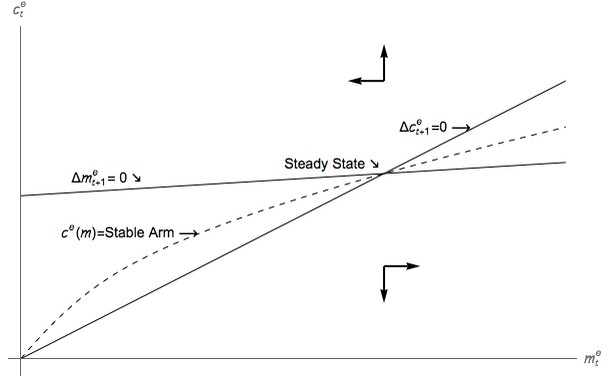
\includegraphics{./Figures/TractableBufferStockPhaseDiag}
\end{figure}
Figure~\ref{fig:PhaseDiag} presents the phase diagram of system
\eqref{eq:DceEq0}-\eqref{eq:xDelEqZero} under our baseline paramete
values. Since the employed consumer never borrows, market resources never fall below the value of current labor income, which is the value selected for the origin of the diagram.\footnote{Our parameterization is not indended to maximize
  realism, but instead to generate well-proportioned figures that
  illustrate the mechanisms of the model as clearly as possible.  The
  parameter values are encapsulated in the file
  \texttt{ParametersBase.m} in the online archive.} 
An intuitive interpretation is that the $\Delta \mRatE_{\tSS} = 0$ locus
characterized by~\eqref{eq:xDelEqZero} shows how much consumption
$\cRatE_{\tNow}$ would be required to leave resources $\mRatE_{\tNow}$
unchanged so that $\mRatE_{\tSS}=\mRatE_{\tNow}$.\footnote{Some
  authors refer to $\Delta \mRatE_{\tSS} = 0$ as the level of
  `permanent income.' However, this definition differs from
  \cite{friedmanATheory}'s and, moreover, is a potential source of
  confusion with permanent labor income' $\Wage_{t} \labor_{t}$; we
  prefer to describe the locus as depicting the level of `sustainable
  consumption.'} 
Thus, any point below the $\Delta \mRatE_{\tSS}=0$
line would have consumption below the break-even amount, implying that
wealth would rise. Conversely for points above $\Delta
\mRatE_{\tSS}=0$. This is the logic behind the horizontal arrows of
motion in the diagram: Above $\Delta \mRatE_{\tSS}=0$ the arrows point
leftward, below $\Delta \mRatE_{\tSS}=0$ the arrows point rightward.

The intuitive interpretation of the $\Delta \cRatE_{\tSS}=0$ locus characterized by~\eqref{eq:DceEq0} is  more subtle. 

Note first that expected consumption growth depends on the amount by
which consumption would fall if the unemployment state were realized,
an amount which depends on the $\cRatE_{\tSS}/\cRatU_{\tSS}$
ratio. For any level of resources, the further below the break-even
level actual consumption is, the smaller the
$\cRatE_{\tSS}/\cRatU_{\tSS}$ ratio is, and therefore the smalle
consumption growth is. Thus, points below the $\Delta \cRatE_{\tSS}=0$
locus are associated with negative values of $\Delta \cRatE_{\tSS}$
(and points above it are associated with positive values). This is the
logic behind the vertical arrows of motion in the diagram: Above the
$\Delta \cRatE_{\tSS}=0$ locus the arrows point upward; below the
$\Delta \cRatE_{\tSS}=0$ locus the arrows point downward.

The slope of the locus depends essentially on the degree of
impatience, as can be seen most directly by considering
\eqref{eq:DcSlope}.  As $\urate$ approaches zero, the proportionality
between $\cE$ and $\mE$ approaches $\pi=1$; this is because the
vanishing risk of unemployment makes borrowing against future income
more and more tempting, and (given our assumption of impatience), the
target level of wealth will approach closer and closer to its minimum
feasible value on the 45 degree line.  On the other hand, as $\urate$
approaches 1 (so that receiving future income becomes more and more
unlikely) the temptation exerted by that future income diminishes, so
the pressure of impatience is smaller and the target level of wealth
is greater.  While the interactions between the terms in
\eqref{eq:DcSlope} are nonlinear, a similar story can be told for the
other indicators of impatience: Greater impatience tilts the slope of
the curve upward, and vice versa.

\begin{figure}
\caption{The Consumption Function for the Employed Consumer}\label{fig:cFunc}
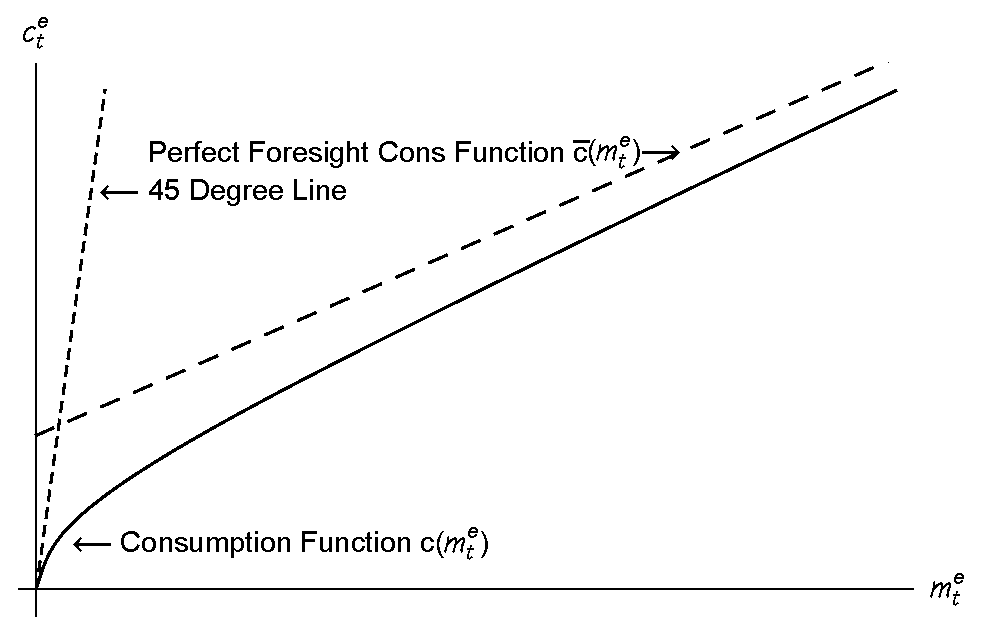
\includegraphics{./Figures/TractableBufferStockcFunc}
\end{figure}

\subsubsection{The Consumption Function \label{sec:consumptionfunction} }
Figure~\ref{fig:cFunc} shows the optimal consumption function $\cFunc(\mRat)$ for an employed consumer (dropping the $e$ superscript to reduce clutter). This is of course the stable arm of the phase diagram. Also plotted are the 45 degree line along which $\cRat_{t} = \mRat_{t}$ and 
\begin{eqnarray}
\label{eq:norisk-consumption}
  \bar{\cFunc}(\mRat) & = & \MPCU(\mRat-1+\hRat),
\end{eqnarray}
where
\begin{eqnarray*}
  \hRat & = & \left(\frac{1}{1-\WGroPF/\Rfree}\right)
\end{eqnarray*}
is the level of (normalized) human wealth.   $\bar{\cFunc}(\mRat)$ is the solution to the no-risk (perfect foresight) version of the model; it is depicted in order to introduce another property of the model: As wealth approaches infinity, the solution to the problem with risky labor income approaches the solution to the no-risk problem arbitrarily closely.\footnote{This limiting result requires that we impose the additional assumption $\PGro < \Rfree$, because the no-risk consumption function is not defined if $\PGro \geq \Rfree$.
}$^{,}$\footnote{If the horizontal axis is stretched far enough, 
  the two consumption functions appear to merge (visually), 
  with the 45 degree line merging (visually) with the vertical axis. 
  The current scaling is chosen both for clarity and 
  to show realistic values of wealth.}


The consumption function $\cFunc(\mRat)$ is \textit{concave}: The marginal
propensity to consume $\MPCFunc(\mRat) \equiv d \cFunc(\mRat)/d \mRat$
is higher at low levels of $m$ because the intensity of the
precautionary motive increases as resources $\mRat$
decline.\footnote{\cite{carroll&kimball:concavity} prove that the
  consumption function must be concave for a general class of
  stochastic processes and utility functions -- including almost all
  commonly-used model assumptions except for the knife-edge cases
  explicitly chosen to avoid concavity.}  The MPC is higher at lowe
levels of $\mRat$ because the \textit{relaxation} in the intensity of the
precautionary motive induced by a small increase in $\mRat$
\citep{kimball:smallandlarge} is relatively larger for a consumer who
starts with less than for a consumer who starts with more resources
\citep{carroll&kimball:concavity}. 

To see this important point, consider a counterfactual. 
Suppose the consumer were to spend all his resources
in period $t$, i.e. $c_{t}=\mRat_{t}$. In this situation, if the
consumer were to become unemployed in the next period, he would then
be left with resources $\mU_{t+1}=(\mRat_{t}-c_{t})\Rfree/\PGro=0$
, which would induce consumption $\cU_{t+1}= \MPCU \mU_{t+1}=0$, yielding
negative infinite utility. A rational, optimizing consumer will always
avoid such an eventuality, no matter how small its likelihood may
be. Thus the consumer never spends all available resources.\footnote{This
  is an implication not just of the CRRA utility function used here
  but of the general class of continuously differentiable utility
  functions that satisfy the \textit{Inada condition} $\uFunc^{\prime}(0)
  = \infty$.}
This implication is illustrated in figure~\ref{fig:cFunc} by the
fact that consumption function always remains below the 45 degree
line.

\subsubsection{Expected Consumption Growth Is Downward Sloping in $\mRatE$}
Figure~\ref{fig:GrowthA} illustrates some of the key points in a different way. It depicts the growth rate of consumption $\cLevE_{t+1}/\cLevE_{t}$ as a function of $\mRatE_{t}$. Consumption growth is equal to what it would be in the absence of risk, plus a precautionary term; for algebraic verification, 
multiply both sides of~\eqref{eq:cedel} by $\PGro$ to obtain:
\begin{eqnarray}
  \left(\frac{\cLevE_{t+1}}{\cLevE_{t}}\right) & = &
  %(\Rfree\Discount)^{1/\CRRA}
  \Pat
   \left\{1+\urate\left[\left(\frac{\cRatE_{t+1}}{\cU_{t+1}}\right)^{\CRRA}-1\right]\right\}^{1/\CRRA}
\label{eq:euler}
.
\end{eqnarray}
Observe that the contribution of the precautionary motive becomes arbitrarily large as $\mRat_{t} \rightarrow 0$, because $\cU_{t+1} = \MPCU\mU_{t+1}  = (\mRat_{t}-\cFunc(\mRat_{t}))\MPCU\Rfree/\PGro$ approaches zero as $\mRat_{t} \rightarrow 0$; that is, as resources $\mRatE_{t}$ decline, expected consumption growth approaches infinity. The point where consumption growth is equal to income growth is at the target value of $\mRatE$.

\begin{figure}
\caption{Income and Consumption Growth}\label{fig:GrowthA}
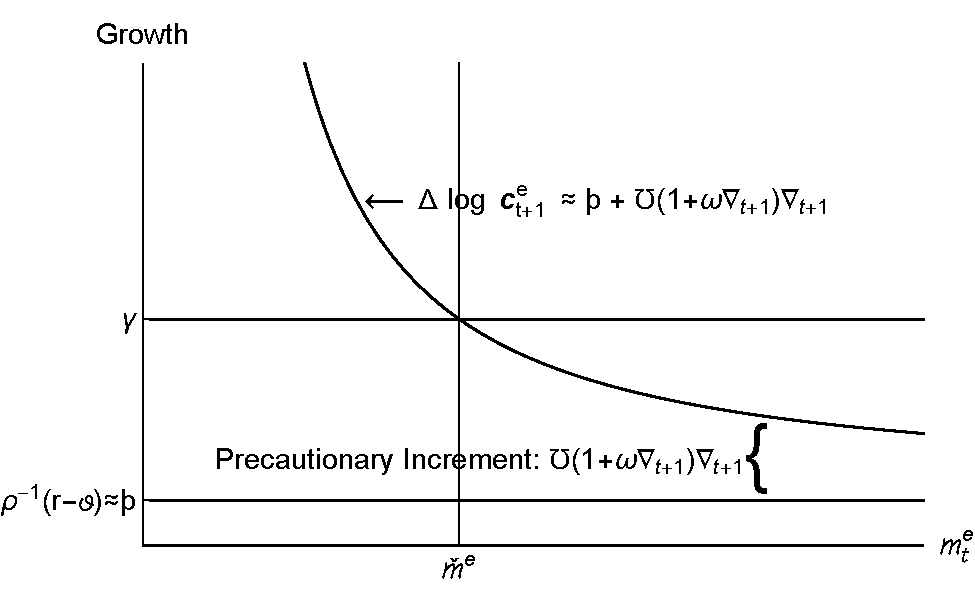
\includegraphics{./Figures/TractableBufferStockGrowthA}
\end{figure}

\subsubsection{Summing Up the Intuition}
We are finally in position to get an intuitive understanding of how
the model works and why a target wealth ratio exists.  On the one
hand, consumers are growth-impatient: It cannot be optimal for them to
let wealth become arbitrarily large in relation to income.  On the
other hand, the precautionary motive intensifies as
the level of wealth falls. The two effects work in opposite
directions. As resources fall, the precautionary motive becomes
stronger, eventually offsetting the impatience motive. The point at
which prudence becomes exactly large enough to match impatience defines
the target wealth-to-income ratio.

\begin{figure}
\caption{Effect of an Increase in $\rfree$}
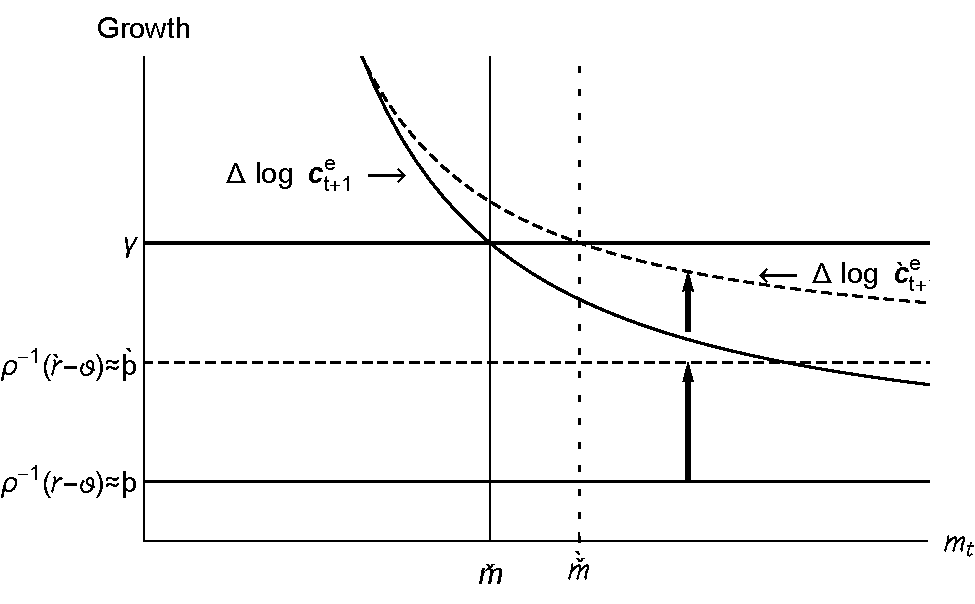
\includegraphics{./Figures/TractableBufferStockGrowthB}
\label{fig:GrowthB}
\end{figure}

It is instructive to work through a couple of comparative dynamics
exercises. In doing so, we assume that all changes to the parameters
are exogenous, unexpected, and permanent.  
Figure~\ref{fig:GrowthB} depicts the effects of increasing 
the interest rate to $\grave{\rfree}>\rfree$.
The no-risk consumption growth locus shifts
up to the higher value $\grave{\patr} \approx
\CRRA^{-1}(\grave{\rfree}-\timeRate)$, inducing a corresponding
increase in the expected consumption growth locus.  Since the expected
growth rate of labor income remains unchanged, the new target level of
resources $\grave{\check{\mRat}}^{e}$ is higher. Thus, an increase in
the interest rate raises the target level of wealth, an intuitive
result that carries over to more elaborate models of buffer-stock
saving with more realistic assumptions about the income process
\citep{BufferStockTheory}.



Figure~\ref{fig:GrowthB} depicts the effects of increasing the risk of unemployment $\urate.$
The principal effect we are interested in is the upward shift in the expected
consumption growth locus to $\Delta \grave{\cLev}_{t+1}$.  If the
household starts at the original target level of resources
$\mTarg$, the size of the upward shift at that point is captured by the
arrow originating at $\{\mTarg,\pGro\}$.  

In the absence of other consequences of the rise in $\urate$, the
effect on the target level of $\mRat$ would be unambiguously positive.
However, recall our adjustment to the growth rate conditional upon
employment~\eqref{eq:meanPreserve}; this induces the shift in the
income growth locus to $\grave{\pGro}$ which has an offsetting effect
on the target $\mRat$ ratio.  Under our benchmark parameter values,
the target value of $\mRat$ is higher than before the increase in risk
even after accounting for the effect of higher $\pGro$, but in
principle it is possible for the $\pGro$ effect to dominate the direct
effect.  Note, however, that even if the target value of $\mRat$ is
lower, it is possible that the \textit{saving rate} will be higher; this
is possible because the higher $\pGro$ makes a given saving
rate translate into a lower ratio of wealth to income.  In any case,
our view is that most useful calibrations of the model are those fo
which an increase in uncertainty results in either an increase in the
saving rate or an increase in the target ratio of resources to
permanent income.  This is partly because our intent is to use the
model to illustate the general features of precautionary behavior,
including the qualitative effects of an increase in the magnitude of
transitory shocks, which unambiguously increase both target $\mRat$
and saving rates.


\begin{figure}
\caption{Effect of an Increase in Unemployment Risk $\urate$ to $\grave{\urate}$}
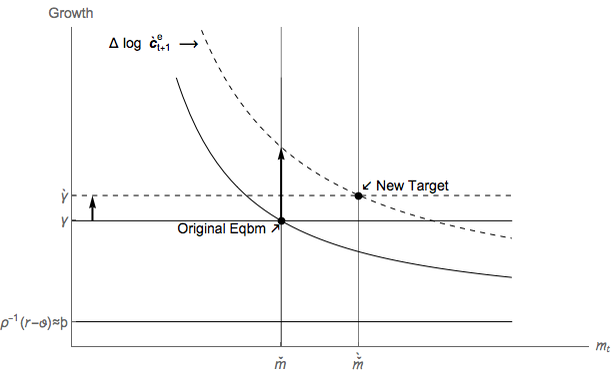
\includegraphics{./Figures/cGroIncreaseMhoPlot}
\label{fig:cGroIncreaseMhoPlot}
\end{figure}


\subsubsection{Death to the Log-Linearized Consumption Euler Equation!\label{sec:death}}
Our simple model may help explain why the attempt to estimate preference
parameters like the degree of relative risk aversion or the time
preference rate using consumption Euler equations has been so signally
unsuccessful \citep{carroll:death}. On the one hand, as illustrated
in figures~\ref{fig:GrowthA} and~\ref{fig:GrowthB}, the steady state
growth rate of consumption, for impatient consumers, is equal to the
steady-state growth rate of income,
\begin{eqnarray}
        \Delta \log ~ \cLevE_{t+1} & = & \pGro. \label{eq:ceqg}
\end{eqnarray}
On the other hand, under logarithmic utility our approximation of the Euler equation for consumption growth, obtained from equation~\eqref{eq:euler}, seems to tell a different story,
\begin{eqnarray}
         \Delta \log ~\cLevE_{t+1} & \approx & \pat +  \urate \nabla _{t+1}, \label{eq:cdelapprox2}
\end{eqnarray}
where the last line uses the Taylor approximations used to obtain~\eqref{eq:cedelapprox}.
The approximate Euler equation~\eqref{eq:cdelapprox2} does not contain any term \textit{explicitly} involving income growth. How can we reconcile~\eqref{eq:ceqg} and~\eqref{eq:cdelapprox2} and resolve the apparent contradiction? The answer is that the size of the precautionary term $\urate \nabla_{t+1}$
is \textit{endogenous} (and depends on $\pGro$). To see this, solve~\eqref{eq:ceqg}-
\eqref{eq:cdelapprox2}: In steady-state,

\begin{eqnarray}
        \urate \nablaTarg & \approx & \pGro - \pat. \label{eq:prectermSS}
\end{eqnarray}
The expression in~\eqref{eq:prectermSS} helps to understand the relationship between
the model parameters and the steady-state level of wealth. From figure~\ref{fig:GrowthA} it is apparent that $\nabla_{t+1}(\mRatE_{t})$ is a downward-sloping function of $\mRatE_{t}$. At low levels of current wealth, much of the spending of an employed consumer is financed by current income.  In the event of job loss, such a consumer must suffer a large drop in consumption, implying a large value of $\nabla_{t+1}$.

To illustrate further the workings of the model, consider an increase in the growth rate of income. On the one hand, the right-hand side of~\eqref{eq:prectermSS} rises. But, lower wealth raises consumption risk, so that the new target level of $\mTarg^{\null}$ must be lower, and this raises the left-hand side of~\eqref{eq:prectermSS}. In equilibrium, both sides of the expression rise by the same amount. 

The fact that consumption growth equals income growth in the steady-state poses major problems for empirical attempts to estimate the Euler equation.  To see why, suppose we had a collection of countries indexed by $i$, identical in all respects except that they have different interest rates $\rfree^{i}$. In the spirit of \cite{hallSubstitution}, one might be tempted to estimate an equation of the form
\begin{eqnarray}
        \Delta \log ~ \cLev^{i} & = & \eta_{0} + \eta_{1} \rfree^{i}+\epsilon^{i}, \label{eq:regression}
\end{eqnarray}
and to interpret the coefficient on $\rfree^{i}$ as an empirical
estimate of the value of $\CRRA^{-1}$. This empirical strategy will
fail. To see why, consider the following stylized scenario. Suppose
that all the countries are inhabited by impatient workers with optimal
buffer-stock target rules, but each country has a different after-tax
interest rate (measured by $\rfree^{i}$). Suppose that the workers are
not far from their wealth-to-income target, so that $\Delta \log
\cLev^{i} = \pGro^{i}$. Suppose further that all countries have \textit{the same} steady-state income growth rate and \textit{the same}
unemployment rate.\footnote{The key point holds if countries have different growth
  rates; this stylized example is merely an illustration. }

A regression of the form of~\eqref{eq:regression} would return the estimates
\begin{eqnarray*}
        \eta_{0} & = & \pGro  \\
        \eta_{1} & = & 0.
\end{eqnarray*}
The regression specification suffers from an \textit{omitted variable} bias caused by the influence of the (endogenous) $\urate \nabla^{i}$ term. In our scenario, the omitted term is correlated with the included variable $\rfree^{i}$ (and if our scenario is exact, the correlation is perfect). Thus, estimates obtained  from the log-linearized Euler equation specification in~\eqref{eq:regression} will be biased estimates of $\CRRA^{-1}$.  For a thorough discussion of this econometric problem, see \cite{carroll:death}.  For a demonstration that the problem is of pratical importance in (macroeconomic) empirical studies, see \cite{ParkerPrestonPrecaution}.


\begin{comment} 
\subsubsection{Dynamics Following An Increase in Patience}
We now consider a final experiment: Figure~\ref{fig:DecreaseTheta} depicts the effect on consumption of a decrease in the rate of time preference (the change is exogenous, unexpected, permanent), starting from a steady-state position. A decrease in the discount rate (an increase in patience) causes an immediate drop in the level of consumption; successive points in time are reflected in the series of dots in the diagram.  The new consumption path (or consumption function) starts from a lower consumption \textit{level} and has a higher consumption \textit{growth} than before the decrease in $\timeRate$.\footnote{The effect of changes in 
  productivity growth is essentially the same as the effect of an 
  increase the interest rate depicted in figure~\ref{fig:GrowthB}.}%

Consumption eventually approaches the new, higher equilibrium target level. This higher level of consumption is financed, in the long run, by the higher interest income provided by the higher target level of wealth.

Note again, however, that equilibrium steady-state consumption growth is still equal to the growth rate of income (this follows from the fact that there is a steady-state \textit{level} for the \textit{ratio} of consumption to income).  The higher target level of the wealth-to-income ratio is precisely enough to reduce the precautionary term by an amount that exactly offsets the effect of the rise in $-\CRRA^{-1}\timeRate$.

Figures~\ref{fig:mPathAfterThetaDrop} and~\ref{fig:MPCPathAfterThetaDrop} depict the time paths of consumption, market wealth, and the marginal propensity to consume following the decrease in $\timeRate$. The dots are spread out evenly over time to give a sense of the rate at which the model adjusts toward the steady state.
\end{comment}



\section{Applications}

Here we provide some illustrations of how the formulas derived above can be used 
to cleanly answer some questions that would be much more difficult to address 
with traditional techniques.

\subsection{The Interest Elasticity of Saving}

A substantial empirical literature attempted to measure something called `the interest
elasticity of saving' from \cite{wrightInterestElasticity} to
the early 1980s.  The inability of that literature to reach any
consensus led \cite{summersCapTax} and others to turn to theoretical
analysis of the problem.

As those papers showed, in a partial equilibrium infinite horizon
perfect foresight context, the question `what is the interest elasticity of saving' does not have a sensible answer.

In that context, an impatient consumer will run his net worth down to
the sticking point defined by the maximum possible amount that he can
borrow.  If the impatient consumer is constrained to have a
minimum wealth of zero the interest elasticity of saving well
defined: It is zero, because the impatient consumer will remain at
zero wealth for any variation in the interest rate such that he
continues to be impatient.

The only other answer to the question (in this perfect
foresight context) comes from an increase in the interest rate that
switches the agent from being impatient to being patient.  A consume
who is patient (relative to the prevailing interest rate) will
accumulate assets forever, so in principle an arbitrarily small
increment to the interest rate could (eventually) produce an
arbitrarily large increase in wealth.  Effectively, the interest
elasticity of saving in such a case would be infinity.

It is tempting to blame these extreme results on the infinite horizon
assumption.  But \cite{summersCapTax} showed that while the answers
obtainable from finite-horizon (life cycle) models were finite, 
they were still extremely -- implausibly -- large.  

Subsequent numerical solutions showed that for specific combinations
of numerical assumptions the response of saving to interest rates can
be radically muted, compared to the perfect foresight benchmark.
(See, e.g., \cite{carroll:bslcpih} o
\cite{cagettiInterestElasticity}).  But such results are a leading
example of the impenetrability of the numerical literature: Adepts in
the literature are persuaded that the results are correct, but little
intuition emerges.  

In our framework, some progress can be made by thinking carefully
about the results above.  Define the saving rate as the amount of saving divided by market
resources $\mLevE$ i.e.\ the personal saving rate out of current
disposable income. Saving is simply market resources minus
consumption. Thus, the saving rate is given by:
\begin{align}
\sRatE_{t} & = \frac{\mLevE_{t}-\cLevE_{t}}{\mLevE_{t}} = 1-\cLevE_{t}/\mLevE_{t} = 1 - \pi
\end{align}
where the quantity $\pi$ is defined in \eqref{eq:DcSlope}.

Figures~\ref{fig:sTargetUrateFixedCRRAVaries}
and~\ref{fig:sTargetCRRAFixedUrateVaries} show the value of the target
saving rate $\sRatE$, as the coefficient of relative risk aversion
$\CRRA$ and the transition probability $\urate$ are
varied. Figures~\ref{fig:sElasticityUrateFixedCRRAVaries}
and~\ref{fig:sElasticityCRRAFixedUrateVaries} show the value of the
elasticity of the target saving rate $\sRatE$ with respect to the
interest rate $\Rfree$, as the coefficient of relative risk aversion
$\CRRA$ and the transition probability $\urate$ are varied.

The intuition for these results can be understood be thinking carefully
about $\pi$: [I bet you can figure out something useful to say here!]



\subsection{An Empirical Application \label{sec:empirical} }
The tractable buffer-stock model emphasizes three factors that affect saving and that might vary substantially over time. First, because the precautionary motive decreases with wealth, the saving rate decreases as market resources $\mLev$ increase. Secondly, because an expansion
in the availability of credit reduces the target level of wealth $\mTarg$, the saving rate decreases as credit conditions tighten. Thirdly, because of the precautionary saving motive, the saving rate increases as unemployment risk $\urate$ rises. \cite{cssUSsaving} estimate a structural version of the tractable model on U.S. data for the 1966-2011 period. Their main findings are: increased credit availability accounts for most of the secular decline in the saving rate; the gap between target and actual wealth accounts for the bulk of the business-cycle variation (including an important part attributable to cyclical movements in the precautionary motive). 

The gist of the structural estimation can be captured by a simple, linear reduced-form model:
\begin{align}
\label{eq:cssUSsaving:regression}
s_{t} = 
\gamma_{1}
+ \gamma_{\mLev} \mLev_{t} 
+ \gamma_{\CEA} \CEA_{t} 
+ \gamma_{\EU} \Ex_{t} u_{t+4}
+ \VectorCoeff^{\prime}_{X} \VectorX_{t}
+ \epsilon_{t}
,
\end{align}
where market resources $\mLev$ are measured as the ratio of household net worth to disposable income, lagged by one period; 
where \CEA~ stands for ``Credit Easing Accumulated'', an index measure of credit supply; 
where $u_{t+4}$ is a proxy for $\urate$ based on survey responses to  four-quarter-ahead expected changes in the unemployment rate; 
and where the vector $\VectorX_{t}$ collects other factors outside the scope of the model, e.g.\ demographics, corporate saving, government saving. 
The theory suggests that the regression coefficients should have the following signs:
\begin{align*}
\gamma_{\mLev} < 0, \gamma_{\CEA} < 0, \gamma_{\EU} > 0
,
\end{align*}


Table~\ref{table:cssUSsaving:regression} reports the estimated coefficients from the univariate regression~\eqref{eq:cssUSsaving:regression}. The three coefficients have the predicted signs and are statistically significant. This parsimonious regression captures about $90$ percent of the variation in saving.


The estimated coefficients on net wealth suggest a long-run marginal
propensity to consume of about $1.2$ cents out of a dollar of total
wealth. This estimate is low compared to studies that do not
explicitly account for credit conditions (the usual range of estimates
is about $3-7$ cents). Structural estimates of the model reinforce
these findings, leading \cite{cssUSsaving} to suggest that much of
what the existing literature has interpreted as pure ``wealth
effects'' may instead reflect some combination of precautionary saving
and credit availability.



\subsection{An International Capital Flows Application \label{sec:macro} }
The high saving rates and rapid accumulation of foreign reserves in emerging economies and the associated financial imbalances between regions present economists with a number of puzzles. One interpretation of these global trends is that they reflect, in some important part, a precautionary accumulation against the risks associated with economic and financial globalization, e.g. increased exposure to external demand and supply shocks; increased vulnerability to exchange rate misalignments and sudden stops; international business cycle spillovers and contagion. \cite{cjSOE} build a small-open macroeconomy version of the tractable model of buffer-stock saving to explore some of these ideas. Individuals are matched to a job at birth, face a constant risk of permanent job-loss throughout their working life (equivalent to uncertain retirement), and die with a fixed probability independent of age. In aggregate equilibrium, labor market flows are in balance and there exists a well-defined distribution of wealth. 

Among other things, \cite{cjSOE} analyze the long-run consequences of a fall in the desired stock of wealth outside of the United States. They show that domestic welfare is unambiguously reduced, in both the short and long run. The main effect operates via a decrease in the capital--output ratio: the world interest rate rises, the domestic real wage falls, stimulating exports during the transition, with the resulting stimulus to domestic output insufficient to offset the greater reduction in investment. Foreign welfare is also reduced in the long run, but may increase in the short run for those generations alive when net foreign assets accumulated by previous generations are used to finance the increase in consumption induced by the fall in the desired stock of wealth.


\section{Conclusions}
The core logic of our tractable model of buffer-stock saving, 
despite its simplicity,
emerges in almost every aspect
under more realistic assumptions that allow for 
transitory shocks, permanent shocks, 
and life-cycle labor-market transitions
calibrated to match the details of the household income process, 
but after much more work \citep{BufferStockTheory}.

We hope that the simplicity of our framework will encourage its use 
in analyzing questions that have so fa
side-stepped the role of nonfinancial risk.
For example, \cite{cjSOE} construct a fully articulated model of
international capital mobility for a small open economy using ou
buffer-stock model as the core element.  We can envision a variety of
other purposes the model could serve, including applications to
topical questions such as the effects of risk in a search model of
unemployment.


\clearpage%

\begin{figure}%
\caption{Effect of Lower $\timeRate$ On Consumption Function}%
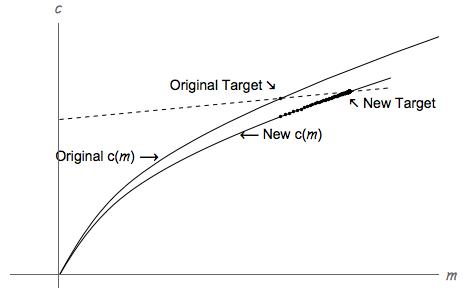
\includegraphics{./Figures/PhaseDiagramDecreaseThetaPlot}%
\label{fig:DecreaseTheta}%
\end{figure}

\begin{figure}%
\caption{Path of $\cRatE$ Before and After $\timeRate$ Decline}%
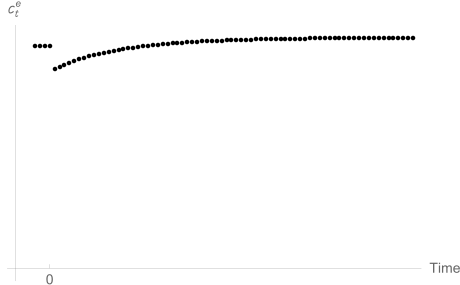
\includegraphics{./Figures/cPathAfterThetaDrop}%
\label{fig:cPathAfterThetaDrop}%
\end{figure}

\begin{figure}%
\caption{Path of $\mRatE$ Before and After $\timeRate$ Decline}%
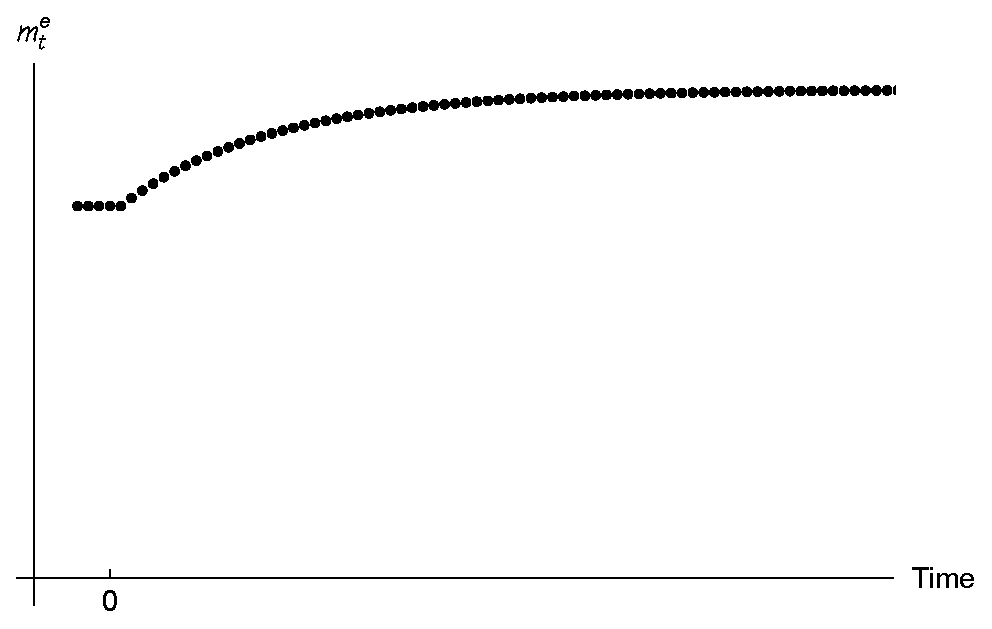
\includegraphics{./Figures/mPathAfterThetaDrop}%
\label{fig:mPathAfterThetaDrop}%
\end{figure}

\begin{figure}%
\caption{Marginal Propensity to Consume $\MPC_{t}$ Before and After $\timeRate$ Decline}%
\medskip%
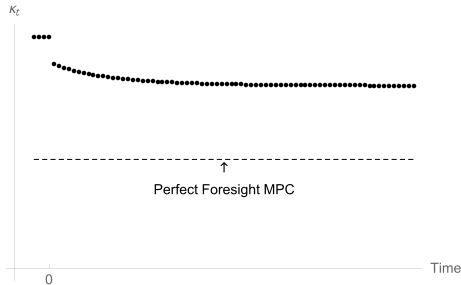
\includegraphics{./Figures/MPCPathAfterThetaDrop}%
\label{fig:MPCPathAfterThetaDrop}%
\end{figure}

\clearpage%

\begin{figure}%
\caption{Target Wealth/Income Ratio, as $\CRRA$ Varies with $\urate$ Fixed}%
\medskip%
\includegraphics{./Figures/mTargetUrateFixedCRRAVaries_4}%
\label{fig:mTargetUrateFixedCRRAVaries}%
\end{figure}

\begin{figure}%
\caption{Target Wealth/Income Ratio, as $\urate$ Varies with $\CRRA$ Fixed}%
\medskip%
\includegraphics{./Figures/mTargetCRRAFixedUrateVaries_4}%
\label{fig:mTargetCRRAFixedUrateVaries}%
\end{figure}

\begin{figure}%
\caption{Marginal Change in Target Ratio, as $\CRRA$ Varies with $\urate$ Fixed}%
\medskip%
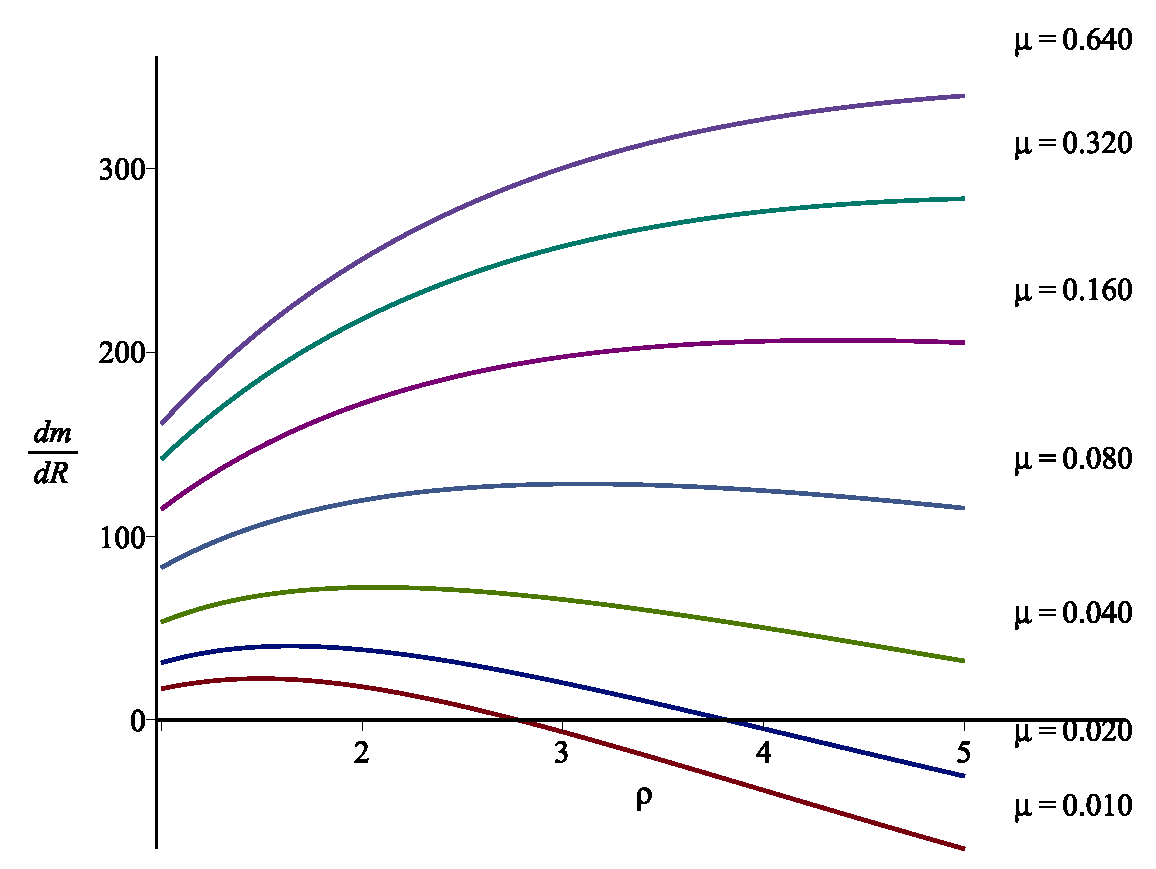
\includegraphics{./Figures/mSlopeUrateFixedCRRAVaries_4}%
\label{fig:mSlopeUrateFixedCRRAVaries}%
\end{figure}

\begin{figure}%
\caption{Marginal Change in Target Ratio, as $\urate$ Varies with $\CRRA$ Fixed}%
\medskip%
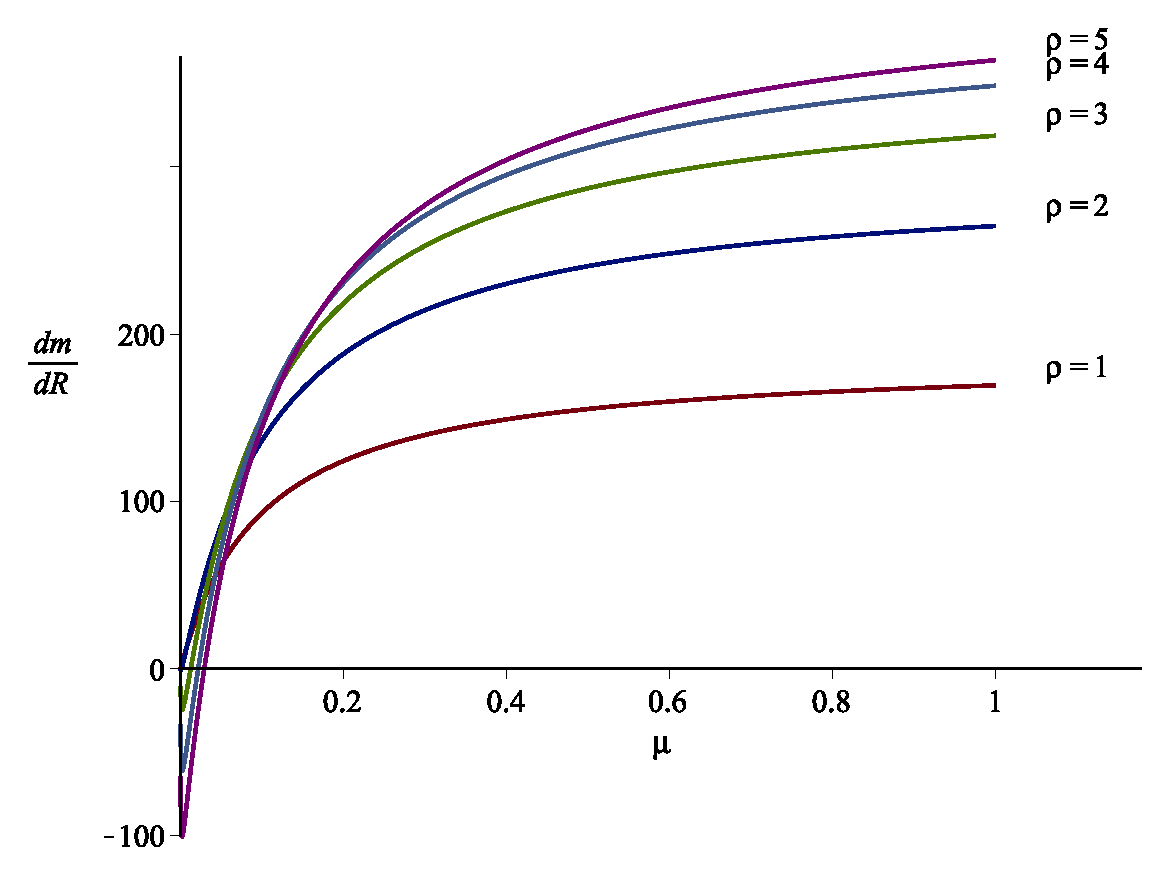
\includegraphics{./Figures/mSlopeCRRAFixedUrateVaries_4}%
\label{fig:mSlopeCRRAFixedUrateVaries}%
\end{figure}

\begin{figure}%
\caption{Target Saving Rate, as $\CRRA$ Varies with $\urate$ Fixed}%
\medskip%
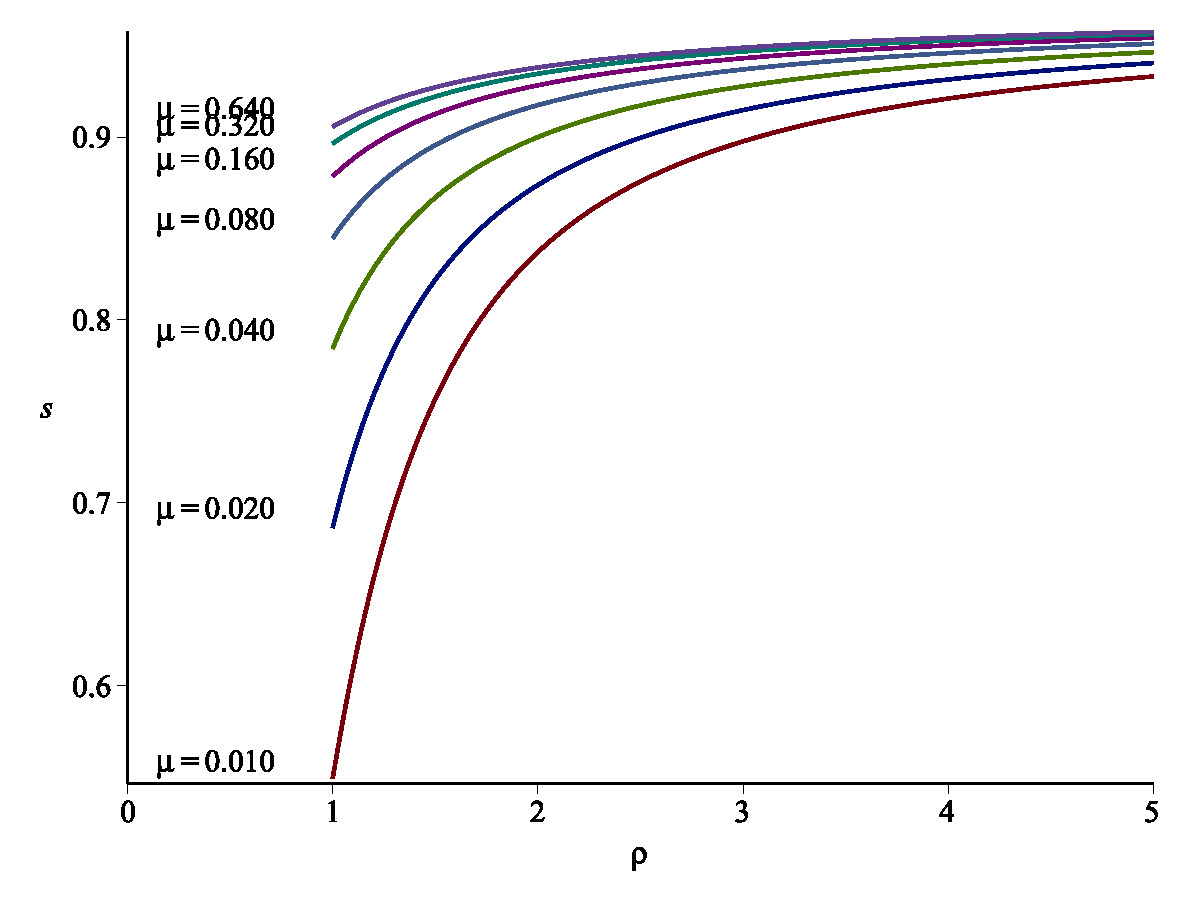
\includegraphics{./Figures/sTargetUrateFixedCRRAVaries_4}%
\label{fig:sTargetUrateFixedCRRAVaries}%
\end{figure}

\begin{figure}%
\caption{Target Saving Rate, as $\urate$ Varies with $\CRRA$ Fixed}%
\medskip%
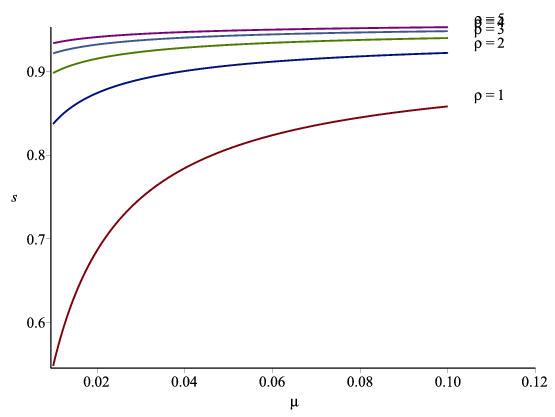
\includegraphics{./Figures/sTargetCRRAFixedUrateVaries_4}%
\label{fig:sTargetCRRAFixedUrateVaries}%
\end{figure}

\begin{figure}%
\caption{Elasticity of Target Saving Rate to changes in the Interest Rate, as $\CRRA$ Varies with $\urate$ Fixed}%
\medskip%
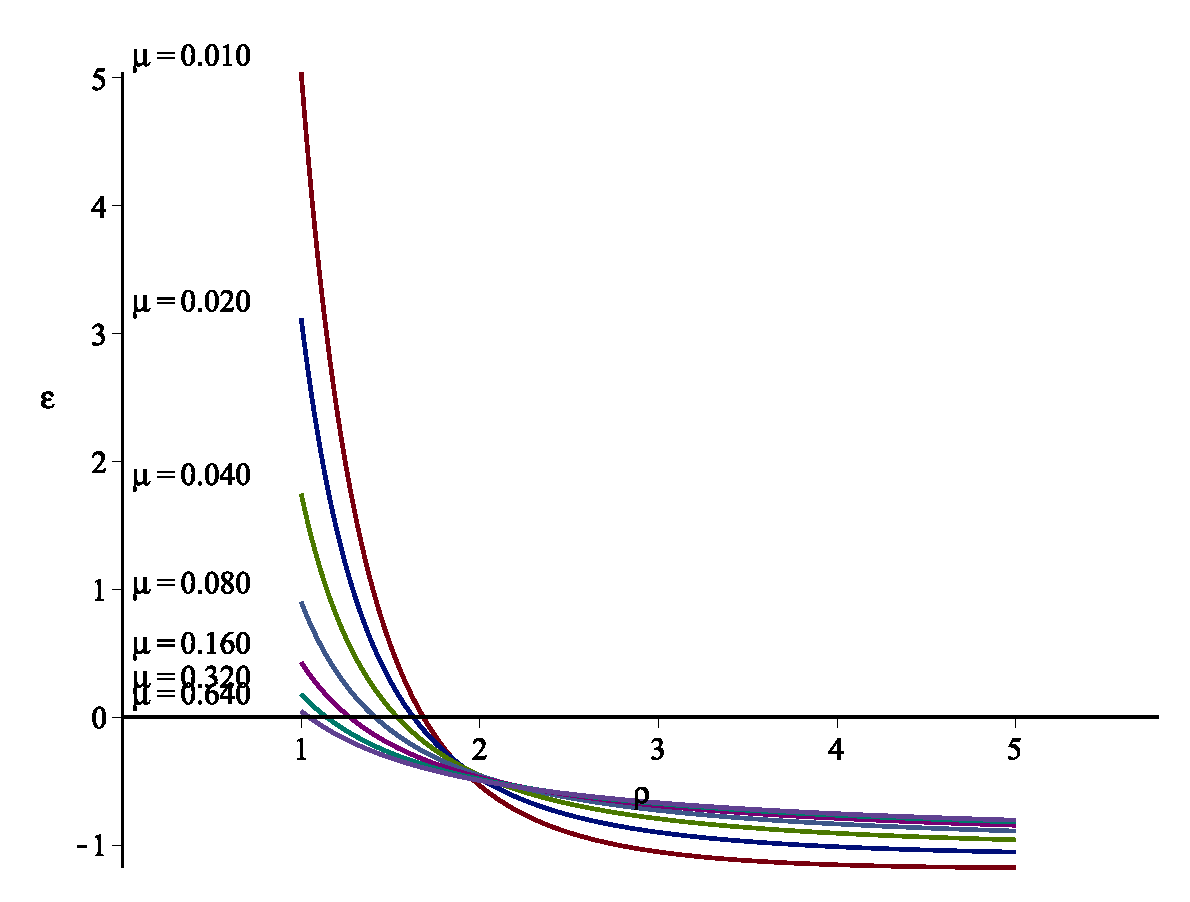
\includegraphics{./Figures/sElasticityUrateFixedCRRAVaries_4}%
\label{fig:sElasticityUrateFixedCRRAVaries}%
\end{figure}

\begin{figure}%
\caption{Elasticity of Target Saving Rate to changes in the Interest Rate, as $\urate$ Varies with $\CRRA$ Fixed}%
\medskip%
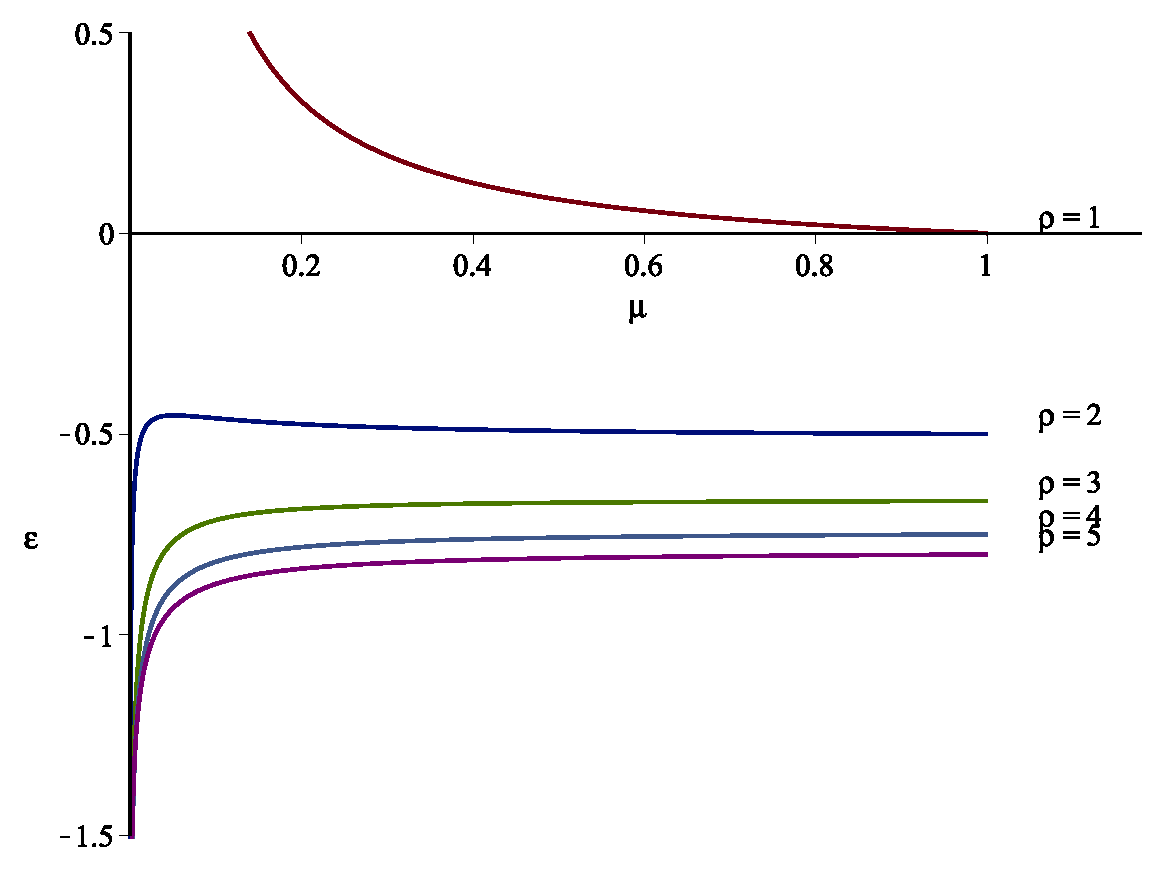
\includegraphics{./Figures/sElasticityCRRAFixedUrateVaries_4}%
\label{fig:sElasticityCRRAFixedUrateVaries}%
\end{figure}



\begin{table}%
\caption{\label{table:mTargetUrateVariesCRRAVaries}}%
\begin{minipage}[b]{0.75\linewidth}%
\centering%
\begin{tabular}{@{}lcccccccc@{}}%
\multicolumn{9}{@{}p{\linewidth}}{\textbf{%
Values of the Target Wealth/Income Ratio as $\CRRA$ and $\urate$ Vary%
}} \cr%
\toprule%
{$\urate$ $\symbol{92}$ $\CRRA$} & 
1 & 2 & 3 & 4 & 5 & 6 & 7 & 8  \cr%
\cmidrule(r){2-9}
0.01        &
2.2 & 6.8 & 11.8 & 16.5 & 20.7 & 24.5 & 28.0 & 31.1 \cr%
0.02        &
3.3 & 9.2 & 15.0 & 20.0 & 24.5 & 28.5 & 32.0 & 35.2 \cr%
0.04        &
5.0 & 12.2 & 18.6 & 24.1 & 28.8 & 33.0 & 36.6 & 39.7 \cr%
0.08        &
7.2 & 15.6 & 22.6 & 28.4 & 33.3 & 37.6 & 41.2 & 44.4 \cr%
0.16        &
9.6 & 18.8 & 26.3 & 32.4 & 37.5 & 41.8 & 45.5 & 48.7 \cr%
0.32        &
11.7 & 21.4 & 29.1 & 35.5 & 40.7 & 45.1 & 48.9 & 52.2 \cr%
0.64        &
13.1 & 23.1 & 31.1 & 37.5 & 42.9 & 47.4 & 51.2 & 54.5 \cr%
\bottomrule\cr%
\multicolumn{9}{@{}l}{%
\parbox{\linewidth}{%
    Source~:~Authors' calculations.
}}\cr%
\end{tabular}%
\end{minipage}
\end{table}
%


\begin{table}%
\caption{\label{table:mSlopeUrateVariesCRRAVaries}}%
\begin{minipage}[b]{0.75\linewidth}%
\centering%
\begin{tabular}{@{}lcccccccc@{}}%
\multicolumn{9}{@{}p{\linewidth}}{\textbf{%
Effect of Cut in After-Tax Interest Rate on Target Ratio (\%)%
}} \cr%
\toprule%
{$\urate$ $\symbol{92}$ $\CRRA$} & 
1 & 2 & 3 & 4 & 5 & 6 & 7 & 8  \cr%
\cmidrule(r){2-9}
0.01         &
6.86  & 2.14  & -1.09 & -2.87 & -3.93 & -4.60 & -5.034 & -5.33  \cr%
0.02         & 
8.65  & 3.64  & .86 & -.71 & -1.69 & -2.35 & -2.81 & -3.13  \cr%
0.04         & 
9.95  & 5.38  & 3.06 & 1.67 & .74 & .07 & -.42 & -.80  \cr%
0.08         & 
10.76  & 7.13  & 5.24 & 4.01 & 3.13 & 2.45  & 1.92  & 1.49  \cr%
0.16         & 
11.21  & 8.60  & 7.08 & 6.00 & 5.17 & 4.50  & 3.96  & 3.50  \cr%
0.32         & 
11.46  & 9.64  & 8.40 & 7.44 & 6.66 & 6.02  & 5.48  & 5.015  \cr%
0.64         & 
11.58  & 10.28  & 9.22 & 8.35 & 7.62 & 7.00  & 6.47  & 6.02  \cr%
\bottomrule\cr%
\multicolumn{9}{@{}l}{%
\parbox{\linewidth}{%
    Source~:~Authors' calculations.
}}\cr%
\end{tabular}%
\end{minipage}
\end{table}

%

\begin{table}%
\caption{\label{table:mTargetUrateVariesCRRAVaries}}%
\begin{minipage}[b]{0.75\linewidth}%
\centering%
\begin{tabular}{@{}lcccccccc@{}}%
\multicolumn{9}{@{}p{\linewidth}}{\textbf{%
Values of the Target Saving Rate as $\CRRA$ and $\urate$ Vary%
}} \cr%
\toprule%
{$\urate$ $\symbol{92}$ $\CRRA$} & 
1 & 2 & 3 & 4 & 5 & 6 & 7 & 8  \cr%
\cmidrule(r){2-9}
0.01         &
.549  & .837 & .898 & .921 & .933 & .941  & .946 & .949 \cr%
0.02         & 
.686  & .874 & .915 & .932 & .941 & .946  & .950 & .953 \cr%
0.04         & 
.784  & .900 & .923 & .940 & .947 & .951  & .954 & .956 \cr%
0.08         & 
.845  & .918 & .937 & .946 & .951 & .954  & .957 & .959 \cr%
0.16         & 
.879  & .928 & .943 & .950 & .954 & .957  & .960 & .960 \cr%
0.32         & 
.896  & .935 & .947 & .953 & .956 & .959  & .961 & .962 \cr%
0.64         & 
.906  & .938 & .949 & .954 & .958 & .960  & .961 & .963 \cr%
\bottomrule\cr%
\multicolumn{9}{@{}l}{%
\parbox{\linewidth}{%
    Source~:~Authors' calculations.
}}\cr%
\end{tabular}%
\end{minipage}
\end{table}
%

\begin{table}%
\caption{\label{table:mTargetUrateVariesCRRAVaries}}%
\begin{minipage}[b]{0.75\linewidth}%
\centering%
\begin{tabular}{@{}lcccccccc@{}}%
\multicolumn{9}{@{}p{\linewidth}}{\textbf{%
Elasticity of the saving Rate to changes in the Interest Rate, as $\CRRA$ and $\urate$ vary%
}} \cr%
\toprule%
{$\urate$ $\symbol{92}$ $\CRRA$} & 
1 & 2 & 3 & 4 & 5 & 6 & 7 & 8  \cr%
\cmidrule(r){2-9}
0.01        &
4.78  & -.60 & -1.08 & -1.16 & -1.17 & -1.17 & -1.16 & -1.15 \cr%
0.02         & 
2.99  & -.52 & -.91 & -1.01 & -1.05 & -1.06 & -1.07 & -1.07 \cr%
0.04         & 
1.68  & -.48 & -.80 & -.90 & -.95 & -.97 & -.99 & -1.00 \cr%
0.08         & 
.87  & -.47 & -.73 & -.83 & -.88 & -.91 & -.93 & -.94 \cr%
0.16         & 
.41  & -.47 & -.69 & -.78 & -.83 & -.86 & -.89 & -.90 \cr%
0.32         & 
.17  & -.48 & -.66 & -.75 & -.80 & -.84 & -.86 & -.88 \cr%
0.64         & 
.046 & -.49 & -.65 & -.74 & -.79 & -.82 & -.84 & -.86 \cr%
\bottomrule\cr%
\multicolumn{9}{@{}l}{%
\parbox{\linewidth}{%
    Source~:~Authors' calculations.
}}\cr%
\end{tabular}%
\end{minipage}
\end{table}
%


\begin{table}%
\caption{\label{table:cssUSsaving:regression}}%
\begin{minipage}[b]{\linewidth}%
\centering%
\begin{tabular}{@{}lccccc@{}}%
\multicolumn{6}{@{}p{\linewidth}}{\textbf{Estimates of the Tractable Model on Post-War U.S. Data}} \cr%
\toprule%
    & {$\gamma_{1}$}
    & {$\gamma_{\mLev}$}
    & {$\gamma_{\CEA}$}
    & {$\gamma_{\EU}$}
    & {Overall} \cr%
\cmidrule(r){2-6}
    & 15.226      & -1.183      &  -6.121     &   0.287     &         \cr%
    & {(}2.157{)} & {(}0.347{)} & {(}0.573{)} & {(}0.075{)} &         \cr%
%    & (2.157) & (0.347) & (0.573) & (0.075) & \cr% doesn't parse inside ()?
$\bar{R}^{2}$ 
    &             &             &             &             &  0.895  \cr%
$p$--value
    &             &             &             &             &  0.000  \cr%
Durbin--Watson
    &             &             &             &             &  0.933  \cr%
\bottomrule\cr% 
\multicolumn{6}{@{}l}{%
\parbox{\linewidth}{%
    Notes~: Estimation sample 1966Q2--2011Q1. 
    Statistically significant at the 1\% level. 
    Newey-West standard errors at $4$ lags.
    Source~:~\cite{cssUSsaving}.
}}\cr%
\end{tabular}%
\end{minipage}
\end{table}

%

\clearpage\newpage
\centerline{\bf \LARGE Appendix}
\renewcommand{\thesection}{A.\arabic{section}}
\setcounter{section}{0}


\section{Taylor Approximation for Consumption Growth}\label{sec:cGroTaylor}
\PTremark{Minor edits in the appendix, mostly presentation. }
Applying a second-order Taylor approximation to \eqref{eq:cedel}, simplifying, and rearranging yields:
\begin{eqnarray*}
        \left\{1+\urate\left[\left(\frac{\cRatE_{t+1}}{\cU_{t+1}}\right)^{\CRRA}-1\right]\right\}^{1/\CRRA} & = & \left\{1+\urate\left[\left(\frac{\cU_{t+1}+\cRatE_{t+1}-\cU_{t+1}}{\cU_{t+1}}\right)^{\CRRA}-1\right]\right\}^{1/\CRRA}
\\      & = & \left\{1+\urate\left[\left(1+\nabla _{t+1}\right)^{\CRRA}-1\right]\right\}^{1/\CRRA}
\\      & \approx &      \left\{1+\urate\left[1+\CRRA \nabla _{t+1}+ \CRRA (\nabla _{t+1})^{2}\prudEx-1\right]\right\}^{1/\CRRA}
\\ & = &         \left\{1+ \CRRA \urate (\nabla _{t+1}+ (\nabla _{t+1})^{2}\prudEx)\right\}^{1/\CRRA}
\\ & \approx & 1+ \urate  \left(1+\nabla _{t+1}\prudEx\right)\nabla _{t+1}. \label{eq:cTaylorRaw}
\end{eqnarray*}


\section{The Exact Formula for $\mTarg^{\null}$}
The steady-state value of $\mRatE$, denoted $\mTarg^{\null}$, is the solution of \eqref{eq:DceEq0}-\eqref{eq:xDelEqZero}, which may be computed in closed form. To simplify some of the intermediate steps in the algebra, define the short-hand notation: 
$\zeta \equiv \Rnorm \MPCU \straight$ and
$\Rnorm \equiv \Rfree\PGro^{-1}$ and 
$\straight\equiv\left(\frac{\PatPGro^{-\CRRA}-\erate}{\urate}\right)^{1/\CRRA}$. From this: $\Rfree \MPCU \straight = \zeta \PGro$.  
A series of straightforward manipulations yields:
\begin{eqnarray}
  \left(\frac{\zeta}{1+\zeta}\right)\mTarg^{\null} & = & (1-\Rnorm^{-1})\mTarg^{\null}+\Rnorm^{-1} \notag
\\  \left(\Rnorm\frac{\zeta}{1+\zeta}\right)\mTarg^{\null} & = & (\Rnorm-1)\mTarg^{\null}+1 \notag
\\  \left(\Rnorm\left\{\frac{\zeta}{1+\zeta}-1\right\}+1\right)\mTarg^{\null} & = & 1 \notag
\\  \left(\Rnorm\left\{\frac{\zeta-(1+\zeta)}{1+\zeta}\right\}+\frac{1+\zeta}{1+\zeta}\right)\mTarg^{\null} & = & 1 \notag
\\  \left(\frac{1+\zeta-\Rnorm}{1+\zeta}\right)\mTarg^{\null} & = & 1 \notag
\\  \mTarg^{\null} & = & \left(\frac{1+\zeta}{1+\zeta-\Rnorm}\right) \notag
\\  \mTarg^{\null} & = & \left(\frac{1+\zeta+\Rnorm-\Rnorm}{1+\zeta-\Rnorm}\right) \notag
\\  \mTarg^{\null} & = & 1 + \left(\frac{\Rnorm}{1+\zeta-\Rnorm}\right) \notag
\\  \mTarg^{\null} & = & 1 + \left(\frac{\Rfree}{\PGro+\zeta\PGro-\Rfree}\right)  \label{eq:mTarget}
.
\end{eqnarray}

A first point about this formula is that:
\begin{eqnarray}
  \zeta\PGro & = & \Rfree \MPCU \left(1+\frac{(\Pat/\PGro)^{-\CRRA} - 1}{\urate}\right)^{1/\CRRA}
\label{eq:zetaPGro}
\end{eqnarray}
is likely to increase as $\urate$ vanishes to zero.\footnote{The effect is
  not necessarily monotonic because $\urate$ affects $\Pat/\PGro$ 
  as well as the denominator of \eqref{eq:mTarget}; however, for
  plausible calibrations the effect of the denominator predominates.}
Note that \eqref{eq:zetaPGro} tends to infinity as $\urate \rightarrow 0$, which implies that $\lim_{\urate \rightarrow 0} \mTarg^{\null} = 1$.  
This is precisely what would be expected since an impatient consumer is self-constrained to keep 
$\mRatE > 1$.  
Thus, as the risk gets infinitesimally small, the
amount by which the target $\mRatE$ exceeds its minimum possible value shrinks to zero.

We now show that the RIC and GIC ensure that the denominator of the fraction in \eqref{eq:mTarget} is positive:
\begin{eqnarray*}
\PGro + \zeta \PGro - \Rfree & = & \PGro + \Rfree \MPCU \straight - \Rfree
 \\& = & \PGro + \Rfree \left(1- \frac{(\Rfree \Discount)^{1/\rho}}{\Rfree}\right) \left(\frac{(\frac{(\Rfree\Discount)^{1/\CRRA}}{\PGro})^{-\CRRA}-1}{\urate}+1\right)^{1/\CRRA}-\Rfree
 \\& > &  \PGro+\Rfree \left(1-\frac{(\Rfree\Discount)^{1/\rho}}{\Rfree}\right)
\left(\frac{(\frac{(\Rfree\Discount)^{1/\CRRA}}{\PGro})^{-\CRRA}-1}{1}+1\right)^{1/\CRRA}-\Rfree
 \\& = & \PGro+\Rfree\left(1-\frac{(\Rfree\Discount)^{1/\rho}}{\Rfree}\right)\frac{\PGro}{(\Rfree\Discount)^{1/\CRRA}}-\Rfree
 \\& = & \PGro+\Rfree \frac{\PGro}{(\Rfree\Discount)^{1/\CRRA}}- \PGro - \Rfree
 \\& = & \Rfree \left(\frac{\PGro}{(\Rfree\Discount)^{1/\CRRA}}-1\right)
 \\& > & 0.
\end{eqnarray*}


\section{An Approximation for $\mTarg^{\null}$}
We can obtain further insight into \eqref{eq:mTarget} by using a judicious mix of first- and second-order Taylor expansions. Define the short-hand $\aleph$:
\begin{eqnarray*}
%\aleph & = & \left(\frac{(\Pat/\PGro)^{-\CRRA} - 1}{\urate}\right)
\aleph & = & \frac{(\Pat/\PGro)^{-\CRRA} - 1}{\urate}%removed brackets
.
\end{eqnarray*}
First, substituting $\MPCU = -\patr$ into \eqref{eq:mTarget}, and computing a second-order Taylor expansion:
\begin{eqnarray}
  \label{eq:zetaExp}
  \zeta\PGro & = & \Rfree \MPCU \left(1+\aleph\right)^{1/\CRRA} \notag
\\ & \approx & -\Rfree \patr \left(1+\CRRA^{-1}\aleph+(\CRRA^{-1})(\CRRA^{-1}-1)(\aleph^{2}/2)\right) \notag
\\ & = & -\Rfree \patr \left(1+\CRRA^{-1}\aleph\left\{1+\left(\frac{1-\CRRA}{\CRRA}\right)(\aleph/2)\right\}\right)
. \label{eq:zetaTaylor2}
\end{eqnarray}

Secondly, applying a first-order Taylor expansion to $\aleph$:
\begin{eqnarray}
\label{eq:hatpi}
\aleph = \frac{(1+\patpGro)^{-\CRRA}-1}{\urate} 
\approx \frac{1- \CRRA \patpGro-1}{\urate}
= -\frac{\CRRA \patpGro}{\urate}
.
\end{eqnarray}
Thirdly, substitute \eqref{eq:hatpi} into \eqref{eq:zetaTaylor2}:
\PTremark{removed a line in the equation below (a reminder of signs of different components is not necessary here, is it?):}
\begin{eqnarray}
  \zeta\PGro 
& \approx &  
-\Rfree \patr \left(1-(\patpGro/\urate)(1+(1-\CRRA)(-\patpGro/\urate)/2)\right)\\ 
%& \approx & 
%\underbrace{-\Rfree \patr}_{>0} \notag \left\{1 / \underbrace{-(\patpGro/\urate)}_{>0}\left(1+\underbrace{(1-\CRRA)}_{<0}\underbrace{(-\patpGro/\urate)}_{>0}/2\right)\right\} 
\label{eq:zetaGammaApprox}
.
\end{eqnarray}
By our definition of $\prudEx$ (the excess of prudence over the logarithmic benchmark):
\begin{eqnarray}
%  \prudEx & \equiv & \left(\frac{\CRRA-1}{2}\right)
  \prudEx & \equiv & \frac{\CRRA-1}{2}%removed brackets
.   \notag
\end{eqnarray}
Equation~\eqref{eq:mTarget} can then be approximated by:
\begin{eqnarray}
 \mTarg^{\null} & \approx & 1 + \left(\frac{1}{\PGro/\Rfree-\patr \left(1-(\patpGro/\urate)(1-(-\patpGro/\urate)\prudEx) \right)-1}\right) \notag
\\ & \approx & 1 + \left(\frac{1}{(\pGro-\rfree)+(-\patr) \left(1+(-\patpGro/\urate)(1-(-\patpGro/\urate)\prudEx)\right)}\right)
\label{eq:mTargetApprox}
\end{eqnarray}
where negative signs have been preserved in front of the $\patr$ and $\patpGro$ terms as a reminder that
the GIC and the RIC imply these terms are themselves negative (so that $-\patr$ and $-\patpGro$ are positive).
An increase in relative risk aversion $\CRRA$, \textit{ceteris paribus}, raises $\prudEx$ and thereby lowers the denominator of \eqref{eq:mTargetApprox}.  This reasoning suggests that
greater risk aversion results in a larger target level of wealth.\footnote{``Suggests'' rather than proves, because
this derivation uses approximations; plausible numerical calibrations are in agreement with the suggestion.}

The formula also provides insight about how the human wealth effect
works in equilibrium.  All else equal, the human wealth effect is captured
by the $(\pGro-\rfree)$ term in the denominator of \eqref{eq:mTargetApprox}:
it is obvious that a larger value of $\pGro$ results in a smaller
target value for $m$.  However, the size of the human wealth
effect also depends on the magnitude of the patience and prudence contributions to the denominator, and those terms could dominate the human wealth effect.  
%This reduction in the human wealth effect is interesting because practitioners have known at least since \cite{summersCapTax} that the human wealth effect is implausibly large in the perfect foresight model.

For \eqref{eq:mTargetApprox} to make sense, we need
the denominator of the fraction to be positive. Let:
\begin{eqnarray}
  \patpGrohat & \equiv & \patpGro(1-(-\patpGro/\urate)\prudEx)
.
\end{eqnarray}
The denominator of \eqref{eq:mTargetApprox} is positive if:
\begin{eqnarray}
  (\pGro - \rfree) & > & \patr - \patr\patpGrohat/\urate \notag
%\\   & = & 
\left(\CRRA^{-1}(\rfree-\timeRate)-\rfree\right)-  \patr\patpGrohat/\urate \notag
\\ \Rightarrow \pGro & > & \CRRA^{-1}(\rfree-\timeRate)-  \patr\patpGrohat/\urate \notag
%\\ 0 & > & \underbrace{\CRRA^{-1}(\rfree-\timeRate) - \pGro}_{<0} -  \patr\patpGrohat/\urate \notag
%\\ \Rightarrow 0 & > & \underbrace{\CRRA^{-1}(\rfree-\timeRate) - \pGro}_{\patpGro} -  \patr(\patpGrohat/\urate) \notag
\\ \Rightarrow 0 & > & \CRRA^{-1}(\rfree-\timeRate) - \pGro -  \patr(\patpGrohat/\urate) \notag
\\ \Rightarrow 0 & > & \patpGro -  \patr(\patpGrohat/\urate) \label{eq:newDenom}
.
\end{eqnarray}
From the RIC, we have $\patr<0$; from the GIC, we have $\patpGro<0$; the latter in turn gives $\patpGrohat < 0$; and thus condition \eqref{eq:newDenom} holds.
\PTremark{I shortened the footnote, might it be removed altogether? I couldn't follow it very well, I wasn't sure what ``the above'' was referring to.}
\footnote{We implicitly assume that, in the second-order Taylor approximation in \eqref{eq:zetaTaylor2}, the absolute value of the second-order term is negligeable relative to the first-order term, i.e. $|\CRRA^{-1} \aleph | \geq |(\CRRA^{-1})(\CRRA^{-1}-1)(\aleph^{2}/2)|$.}
%\footnote{In more detail: For the second-order Taylor approximation in \eqref{eq:zetaTaylor2}, we implicitly assume that the absolute value of the second-order term is negligeable relative to the first-order term, i.e. $|\CRRA^{-1} \aleph | \geq |(\CRRA^{-1})(\CRRA^{-1}-1)(\aleph^{2}/2)|$. Substituting \eqref{eq:hatpi}, the above could be simplified to $1 \geq (-\patpGro/\urate)\prudEx$, therefore we have $\patpGrohat < 0$. This simple justification is based on the proof above that RIC and GIC guarantee the denominator of the fraction in \eqref{eq:mTarget} is positive.}

The same set of derivations imply that we can
replace the denominator in \eqref{eq:mTargetApprox} with the negative
of the RHS of \eqref{eq:newDenom}, yielding a more compact expression
for the target level of resources:
\begin{eqnarray} 
 \mTarg^{\null} & \approx & 1 + \left(\frac{1}{\patr(\patpGrohat/\urate) - \patpGro }\right) \notag
\\ & = & 1 + \left(\frac{1/(-\patpGro)}{1+(-\patr/\urate)(1+(-\patpGro/\urate)\prudEx)  }\right) \label{eq:mTargetCompact}
.
\end{eqnarray}
This formula makes plain that an
increase in either form of impatience raises the denominator of the 
fraction in 
\eqref{eq:mTargetCompact} and thus reduces the target level of assets.

Two specializations of the formula are particularly useful.  The first useful special case is $\CRRA = 1$ (logarithmic utility).  In this case,
\begin{eqnarray*}
  \prudEx & = & 0
\\  \patr & = & -\timeRate
\\  \patpGro & = & \rfree-\timeRate-\pGro
%\\  \patpGrohat & = & -\pGro
\end{eqnarray*}
and the approximation reduces to:
\begin{eqnarray}
 \mTarg^{\null} & \approx & 1 + \left(\frac{1}{(\pGro-\rfree)+\timeRate(1+(\pGro+\timeRate-\rfree)/\urate)}\right)
\label{eq:mTargetCompactLogUtility}
\end{eqnarray}
Equation \eqref{eq:mTargetCompactLogUtility} neatly captures the effect of an increase in human wealth (an increase in $\pGro$ or a decrease in $\rfree$), the effect of an increase in impatience $\timeRate$, 
the effect of a decrease in unemployment risk $\urate$: these reduce target wealth.


The second useful special case is $\rfree = \timeRate$ (but $\CRRA>1$).  In this case,
\begin{eqnarray*}
    \patr & = & -\timeRate
\\  \patpGro & = & -\pGro
\\  \patpGrohat & = & -\pGro (1-(\pGro/\urate)\prudEx)
\end{eqnarray*}
and the approximation becomes:
\begin{eqnarray}
 \mTarg^{\null} & \approx & 1 + \left(\frac{1}{(\pGro-\rfree)+\timeRate(1+(\pGro/\urate)(1-(\pGro/\urate)\prudEx))}\right)
 \label{eq:mTargetCompactNeutralPatience}
\end{eqnarray}
Equation~\eqref{eq:mTargetCompactNeutralPatience} shows that an increase in the prudence term $\prudEx$
shrinks the denominator and thereby boosts the target level of
wealth.\footnote{It would be inappropriate to use the equation to
  consider the effect of an increase in $\rfree$ because the equation was derived under the
  assumption $\timeRate=\rfree$, so $\rfree$ is not free to vary.}
 %contains the appendix

\clearpage\newpage

\begin{table}
\caption{Summary of Notation}
\label{table:notation}
\medskip\medskip
\begin{tabular}{rcl}
    $a$                            & - & end-of-period $t$ assets (after consumption decision)
\\  $b$                            & - & middle-of-period $t$ balances (before consumption decision)
\\  $c$                            & - & consumption
\\  $\ell$                         & - & personal labor productivity 
\\  $m$                            & - & market resources (capital, capital income, and labor income)
\\  $\Rfree$, $\rfree$             & - & interest factor, rate 
\\  $\Wage$                        & - & aggregate wage
\\  $\WGro$                        & - & growth factor for aggregate wage rate $\Wage$
\\  $\PGro\equiv\WGro/(1-\urate)$  & - & conditional (on employment) growth factor for individual labor income
\\  $\pGro$                        & - & $\log \PGro$, conditional growth {\it rate} for labor income
\\  $\Discount$                    & - & time preference factor ($=1/(1+\timeRate)$)
\\  $\empState$                    & - & dummy variable indicating the employment state, $\empState\in\{0,1\}$
\\  $\MPC$                         & - & marginal propensity to consume
\\  $\CRRA$                        & - & coefficient of relative risk aversion
\\  $\timeRate$                    & - & time preference rate ($\approx - \log \Discount$)
\\  $\urate$                       & - & probability of falling into permanent unemployment 
%\\  $\erate=1-\urate$              & - & probability of staying in employment from one period to the next
\\  $\Pat$, $\pat$                 & - & absolute patience factor, rate
\\  $\PatPGro$, $\patpGro$               & - & growth patience factor, rate
\\  $\PatR$, $\patr$               & - & return patience factor, rate
\\  $\prudEx$                      & - & excess prudence factor ($=(\CRRA-1)/2$)
\\  $\nabla$                       & - & proportional consumption drop upon entering unemployment
\\  $\Rnorm$                       & - & short for  $\Rfree/\PGro$
%\\  $\straight$                    & - & short for  $\left(\frac{\PatPGro^{-\CRRA}-\erate}{\urate}\right)^{1/\CRRA}$
\end{tabular}
\end{table}
%summarizes the notation



\bibliography{economics,\texname,\texname-Add}

\end{document}
